\documentclass[a4paper,oneside]{Tptesi2}

\usepackage[italian]{babel}
\usepackage{listings}
\usepackage{lmodern} % diverso font
\usepackage{amsmath,amssymb, amsfonts, amsthm}
\usepackage{verbatim}
\usepackage{indentfirst}
\usepackage[utf8]{inputenc}
\usepackage{subfigure}
\usepackage{algorithmic}
\usepackage{framed}
\usepackage{rotating}
\usepackage{cite}
\usepackage{latexsym}
\usepackage{xcolor}
\usepackage{resizegather}

\usepackage{booktabs}
\usepackage{graphicx}


\definecolor{codegreen}{rgb}{0,0.6,0}
\definecolor{codegray}{rgb}{0.5,0.5,0.5}
\definecolor{codepurple}{rgb}{0.58,0,0.82}
\definecolor{backcolour}{rgb}{0.95,0.95,0.92}
 
\lstdefinestyle{mystyle}{
    backgroundcolor=\color{backcolour},   
    commentstyle=\color{codegreen},
    keywordstyle=\color{magenta},
    numberstyle=\tiny\color{codegray},
    stringstyle=\color{codepurple},
    basicstyle=\footnotesize\ttfamily,
    breakatwhitespace=false,         
    breaklines=true,                 
    captionpos=b,                    
    keepspaces=true,                 
    numbers=left,                    
    numbersep=5pt,                  
    showspaces=false,                
    showstringspaces=false,
    showtabs=false,                  
    tabsize=2,
}

\lstset{style=mystyle}

%\lstset{style=mystyle, inputencoding=utf8,extendedchars=true}
%\makeatletter
%\lst@InputCatcodes
%\def\lst@DefEC{%
% \lst@CCECUse \lst@ProcessLetter
%  ^^^^03b1% α
%  ^^^^^^01d6fc% 𝛼
%  ^^^^^^01d45d% 𝑝
%  ^^00}
%\lst@RestoreCatcodes
%\makeatother


% Packages -----------------------------------------------------------------------
%\usepackage{amsthm}
%\usepackage{amsmath}          % Non necessario se usi TPTESI2 perche' gia` incluso
%\usepackage[dvips]{graphicx}  % Non necessario se usi TPTESI2 perche' gia` incluso
%\usepackage{url} %non usare se si usa hyperref


\newcommand{\mr}{\emph{motore di ricerca}}
\newcommand{\Mr}{\emph{Motore di ricerca}}
\newcommand{\ws}{Web~service }


% Use a small font for the verbatim environment
\makeatletter  % makes '@' an ordinary character
\renewcommand{\verbatim@font}{%
  \ttfamily\footnotesize\catcode`\<=\active\catcode`\>=\active%
}
\makeatother   % makes '@' a special symbol again
%
% Simboli Matematici -------------------------------------------------------------
%\newcommand{\h}{\mathcal{H}_\infty} % scorciatoia per sequenza usata spesso
% Definizioni & Teoremi ----------------------------------------------------------
\newtheorem{teorema}{Teorema}[chapter]
\newtheorem{corollario}[teorema]{Corollario}
\newtheorem{lemma}[teorema]{Lemma}
%\theoremstyle{definition}
\newtheorem{definizione}{Definizione}[chapter]
\newtheorem{proposizione}[definizione]{Proposizione}
% Formattazione Figure -----------------------------------------------------------
\setcounter{topnumber}{3}
\setcounter{totalnumber}{3}
\def\topfraction{1}
\def\textfraction{0}
% Fuzz ---------------------------------------------------------------------------
%\hfuzz10cm %Non scassare linee che escono dal bordo
% Frontespizio -------------------------------------------------------------------
       \title{Modello di programmazione lineare intera per la pianificazione di turni ospedalieri}
       \author{Giulia Forasassi}
       \titolocorso{Ingegneria Informatica}
       \chair{Prof. Fabio Schoen\\ }
       \numberofmembers{1} %numero dei relatori
       \degreeyear{2018/2019}
       \numerocorrelatori{2} %numero dei correlatori
       \correlatori{Dott. Matteo Lapucci} % i correlatori separati da \\

%
% ---- Inclusioni (vedi piu` sotto per il comando "include" --------------
%\includeonly {introduzione,chapter1, chapter2}
%\includeonly {chapter1, chapter2, chapter3, chapter4, chapter5, chapter6}
%\includeonly{chapter6}
%
\hypersetup{%
%  pdfpagemode=FullScreen,%
  plainpages=false,%
  breaklinks,%
  pdftitle={},%
  pdfauthor={},%
  pdfsubject={},%
  pdfkeywords={},%
  colorlinks=false}

\begin{document}

\frontmatter

%\hyphenation{}
%
\pagestyle{headings} % rende attive le impostazioni sulla testata!
%
\maketitle % crea il frontespizio (ricordati di copiare "stemma.eps" nella tua directory)
%
%
%\pagenumbering{roman}
\tableofcontents % inserisce indice generale
\cleardoublepage
%\addcontentsline{toc}{chapter}{Elenco delle figure}
%\listoffigures   % inserisce indice figure
%\addcontentsline{toc}{chapter}{Elenco delle tabelle}
%\listoftables    % inserisce indice tabelle
%\addcontentsline{toc}{chapter}{Elenco degli algoritmi}
%\listofalgorithms
%
%--------------- Inizio del testo vero e proprio
%

%\cleardoublepage
%\pagenumbering{arabic}
%\chapter*{Ringraziamenti}\label{ch:ringraziamenti}
Per concludere vorrei ringraziare in primis il Professor Fabio Schoen, relatore di questa tesi di laurea, e il Dottor Matteo Lapucci, correlatore, senza i quali questo lavoro non sarebbe stato possibile.\\

Inoltre vorrei ringraziare i miei genitori per avermi sempre sostenuta e per avermi permesso di portare a termine questo primo ciclo dei miei studi universitari, senza farmi mancare mai niente.
Grazie di cuore anche a tutti gli altri componenti della mia famiglia, a mio zio Roberto, e alle mie cugine Chiara e Rebecca, e a tutti i miei amici più fidati.\\

Un ringraziamento sincero al mio amato amico felino, Merlino, che mi ha sempre accompagnata nelle serate di studio intenso.\\

Infine un ringraziamento speciale va al mio ragazzo, Federico, detto anche "Il grande Capo", da cui ho imparato tantissimo, il quale mi ha sempre supportato e sopportato credendo in me anche quando nemmeno io ci credevo. Grazie per ogni singola volta che mi hai aiutata e spronata mostrandomi tutto il tuo amore.\\

\begin{center}
Grazie di cuore a tutti.
\end{center}
\frontmatter

\mainmatter
\chapter{Introduzione}\label{ch:introduzione}
Il lavoro di questa tesi è stato costruire un programma per gestire il \textbf{cambio dei turni del personale infermieristico} all'interno di un ospedale.
Il problema preso in esame è da sempre una questione di fondamentale importanza nell'organizzazione del lavoro all'interno della sanità, e anche in altre realtà lavorative. Quindi, lo scopo di questo progetto è stato creare un \textbf{modello di ottimizzazione} per la pianificazione dei turni lavorativi ospedalieri in modo da trovare una soluzione che soddisfi al meglio i vincoli desiderati.

Il lavoro svolto in questa tesi si basa sui requisiti imposti dalla competizione \textit{Second International Nurse Rostering Competition}, avvenuta tra il 2014 e il 2015 con lo scopo di incoraggiare la ricerca sui metodi automatizzati di selezione degli infermieri per risolvere un problema di assegnamento del personale infermieristico.\\

Si è modellato tale problema come un \textbf{problema di programmazione lineare intera}, le cui variabili sono per la maggior parte binarie. 
Tale programma è stato implementato in Python, usando l'ottimizzatore commerciale Gurobi. Inoltre, una volta creato il modello, sono stati fatti degli esperimenti basandosi su dati reali presi direttamente dalle specifiche della competizione.

La tesi è articolata in \textbf{6 capitoli}, questa introduzione è il primo di essi.
Nel secondo capitolo vengono forniti i contenuti teorici che stanno alla base della programmazione lineare intera. Nel terzo capitolo si introduce il problema in questione spiegando i dati che il programma riceve in input e analizzando nel dettaglio i vincoli del modello creato.
Il quarto capitolo mostra i risultati degli esperimenti fatti sui dati reali, con lo scopo di valutare il modello creato.
Successivamente, nel quinto capitolo si mostra l'interfaccia grafica che permette di utilizzare il modello, realizzata mediante il framework Django.
Infine, nell'ultimo capitolo, vengono tratte le conclusioni di questo lavoro di tesi di laurea.



 
\chapter{Contenuti teorici}\label{ch:chapter1}

\section{Ottimizzazione}
In questo capitolo vengono spiegati i principali concetti teorici che costituiscono il fondamento del problema preso in esame; dapprima si presenteranno le nozioni che stanno alla base di un generale problema di ottimizzazione e successivamente si spiegheranno più nel dettaglio le caratteristiche principali della \textbf{Programmazione Lineare Intera}.

\subsection{Problema di ottimizzazione}
Un problema di ottimizzazione è un problema relativo alla scelta della soluzione migliore, detta \textbf{soluzione ottima}, tra quella disponibili in base ad un determinato criterio. Vi sono tre elementi principali che caratterizzano un problema di ottimizzazione:
\begin{itemize}
\item \textit{le variabili decisionali}: sono variabili di cui si deve determinare il valore ottimo;
\item \textit{l'insieme ammissibile}: è l'insieme delle alternative disponibili per il decisore;
\item \textit{la funzione obbiettivo}: indica la relazione funzionale tra le variabili decisionali e altre variabili il cui valore debba essere massimizzato o minimizzato; cioè, in altre parole, costituisce un criterio di scelta tra le possibili soluzioni del problema con l'intento di selezionare solo quelle migliori, cioè quelle che minimizzano il costo o massimizzano il profitto.
\end{itemize}

Quindi un'istanza di un problema di ottimizzazione è definita come una coppia (A, f), dove A è l'insieme delle soluzioni ammissibili ed $f: A \rightarrow \Re$ è la funzione obbiettivo che si deve ottimizzare (massimizzare o minimizzare).
Il problema di ottimizzazione viene posto chiedendo di trovare i valori $x \in A$ tali che: $f(x) ~ \leq ~ f(y) ~~~ \forall y \in A$  (problema di minimizzazione).
Tali valori x costituiscono delle soluzioni ottime \textbf{globali} per il problema; nel caso in cui risulti invece $f(x) ~ \leq ~ f(y) ~~~ \forall y \in ad ~ un ~ intorno ~ di ~ x$, allora la soluzione x si dice soluzione ottima \textbf{locale}. \\

Nella formulazione di un problema di ottimizzazione un aspetto assai critico e rilevante è costituito dalla corretta definizione dell'insieme delle soluzioni ammissibili; è necessario delimitare questo sottoinsieme dello spazio delle soluzioni, senza escludere punti dello spazio che possano corrispondere ad una soluzione ammissibile e dunque potenzialmente ottima, e al tempo stesso cercando di ridurre al massimo l'insieme entro cui eseguire la ricerca delle soluzioni, per rendere più efficiente e meno oneroso, in termini computazionali, il procedimento di calcolo adottato per individuare le soluzioni ottime. In generale quindi l'insieme A delle soluzioni ammissibili viene definito attraverso un insieme di \textbf{vincoli} che limitano e circoscrivono l'insieme entro cui possono assumere valori le variabili del problema.

In particolare tra i problemi di ottimizzazione rivestono notevole importanza i \textbf{problemi di programmazione matematica} dove i vincoli che circoscrivono l'insieme A delle soluzioni ammissibili sono costituiti da un certo numero, anche molto ampio ma finito, di equazioni o disequazioni. In generale, quindi, un problema di programmazione matematica viene definito come segue:
\begin{equation}
\begin{split}
min ~ &f(x) \\
g_i(x) ~ &\geq ~ 0 ~~~ \forall i \in \{1,..,m\} \\
h_j(x) ~ &= ~ 0 ~~~ \forall i \in \{1,..,p\} \\
\end{split}
\end{equation}
\\
%Infine nel caso in cui il problema, di cui si vuole trovare la soluzione ottima, risulti molto complicato da risolvere può essere utile lavorare mediante il relativo \textbf{problema rilassato} il quale, risulta caratterizzato da un numero minore di condizioni vincolanti rispetto al problema di riferimento, e quindi appare molto più facile da risolvere.


\subsection{Programmazione lineare}
La programmazione lineare è quella branca della Ricerca Operativa che si occupa di studiare algoritmi di risoluzione per problemi di ottimizzazione lineari.
Un problema è detto \textbf{lineare} se sia la funzione obbiettivo sia i vincoli sono funzioni lineari. Questo significa che la funzione obbiettivo può essere scritto come:
\begin{equation}
f ~ = ~ \sum_{i=1}^{N_v} ~ c_i ~ x_i ~ = ~ c^T ~ x 
\end{equation}
avendo indicato con:
\begin{itemize}
\item $N_v$: il numero delle variabili che descrivono il problema;
\item $c$: il vettore colonna dei coefficienti $c_i$ della funzione obbiettivo;
\item $x$: il vettore colonna delle variabili $x_i$;
\item infine la T all'esponente indica l'operatore di trasposizione.
\end{itemize}

Esistono tre grandi classi di problemi lineari:
\begin{enumerate}
\item \textbf{Problemi lineari continui (LP)}: sono problemi che presentano al loro interno solo variabili continue, cioè variabili che possono assumere con continuità tutti i valori contenuti all'interno del loro dominio di esistenza.
Per questi tipi di problemi il principale algoritmo di risoluzione è detto \textit{Algoritmo del Simplesso};
\item \textbf{Problemi lineari interi (ILP)}: sono problemi lineari che presentano al loro interno solo variabili intere, cioè variabili che possono assumere solo i valori interi contenuti all'interno del loro dominio di esistenza.
Per questa classe di problemi esiste un algoritmo di risoluzione molto importante, chiamato \textit{Branch and Bound};
\item \textbf{Problemi lineari misto-interi (MILP)}: sono problemi che al loro interno presentano sia variabili intere che continue. L'algoritmo di risoluzione principale è detto \textit{Branch and Bound}.
\end{enumerate}


\section{Programmazione Lineare Intera}
La Programmazione Lineare Intera tratta il problema della minimizzazione (o massimizzazione) di una funzione lineare di più variabili, soggetta a vincoli di uguaglianza e disuguaglianza lineari ed alla restrizione che tutte variabili possano assumere \textbf{solo valori interi}. Si tratta dunque di problemi del tipo:
\begin{equation}
\begin{split}
& min ~ \sum_{j=1}^n ~ c_j x_j \\
& \sum_{j=1}^n ~ a_{i, j} ~ x_j ~ = ~ b_i ~~~ \forall i \in \{1,...,m\} \\
& x_j ~ \geq ~ 0 ~~~ \forall j \in \{1,...,n\} \\
& x_j ~ \in \mathbb{N} ~~~ \forall j \in \{1,...,n\}
\end{split}
\end{equation}
La stessa formulazione vale nel caso si voglia massimizzare la funzione obbiettivo.

Moltissimi problemi reali possono essere rappresentati da modelli di Programmazione Lineare Intera; tipicamente si tratta di problemi in cui le variabili di decisione rappresentano quantità indivisibili oppure sono problemi caratterizzati dalla necessità di scegliere tra un numero finito di alternative diverse. In quest'ultimo caso, in particolare, si avranno problemi di \textbf{Programmazione Lineare Zero-Uno} o Binaria, cioè problemi in cui le variabili sono binarie e perciò possono assumere solo i valori 0 o 1.


\subsection{Tecniche di modellazione}
In questa sezione vengono presentate alcune tecniche di modellazione che facilitano la formulazione di problemi di programmazione lineare intera.

\subsubsection*{Variabili binarie}
Le variabili binarie vengono usate quando si vuole rappresentare un evento mediante la scelta tra 2 alternative disponibili, cioè:
\begin{equation}
\label{eq:varBinarie}
\delta=
\begin{cases}
1, & \text{se l'evento si verifica,} \\
0, & \text{altrimenti.}
\end{cases}
\end{equation}

\subsubsection*{Vincoli logici}
Siano $A$ e $B$ due eventi e $\delta_A$ e $\delta_B$ le corrispettive variabili di decisione. Esprimiamo condizioni logiche sugli eventi mediante vincoli sulle variabili di decisione corrispondenti.
\begin{enumerate}
\item \textit{And}\\
Supponiamo di avere la seguente condizione logica: $A~\wedge~B$.
Dalla tabella di verità (Tabella \ref{tab:tableAND}) è evidente che questa condizione è soddisfatta quando entrambi gli eventi si sono verificati, e quindi quando entrambe le variabili di decisione relative sono pari ad 1.

\begin{table}[h!]
  \begin{center}
    \begin{tabular}{l|c|c} % <-- Alignments: 1st column left, 2nd middle and 3rd right, with vertical lines in between
      %\textbf{$\delta_A$} & \textbf{$\delta_B$} & \textbf{$A~and~B$}\\
      $\delta_A$ & $\delta_B$ & $A~\wedge~B$ \\
      \hline
      0 & 0 & F\\
      0 & 1 & F\\
      1 & 0 & F\\
      1 & 1 & T\\
    \end{tabular}
    \caption{Tabella di verità: and}
    \label{tab:tableAND}
  \end{center}
\end{table}

Questo equivale ad imporre il seguente vincolo: $\delta_A + \delta_B$.

\item \textit{Or}\\
Supponiamo di avere la condizione logica: $A~\vee~B$.
In questo caso si può vedere che tale condizione è soddisfatta quando almeno uno dei due eventi si è verificato, e quindi quando almeno una delle due variabili è pari ad 1 (Tabella \ref{tab:tableOR}).\\\\

\begin{table}[h!]
  \begin{center}
    \begin{tabular}{l|c|c} % <-- Alignments: 1st column left, 2nd middle and 3rd right, with vertical lines in between
      %\textbf{$\delta_A$} & \textbf{$\delta_B$} & \textbf{$A~and~B$}\\
      $\delta_A$ & $\delta_B$ & $A~\vee~B$ \\
      \hline
      0 & 0 & F\\
      0 & 1 & T\\
      1 & 0 & T\\
      1 & 1 & T\\
    \end{tabular}
    \caption{Tabella di verità: or}
    \label{tab:tableOR}
  \end{center}
\end{table}

Questo equivale ad imporre il seguente vincolo: $\delta_A + \delta_B \geq 1$.
\\
\item \textit{Or esclusivo}\\
Sia la seguente condizione logica: $A~\oplus~B$.
Questa situazione è molto simile a quella appena vista ma, contrariamente a prima, le variabili decisionali non possono essere entrambe pari ad 1 (Tabella \ref{tab:tableORe}).

\begin{table}[h!]
  \begin{center}
    \begin{tabular}{l|c|c} % <-- Alignments: 1st column left, 2nd middle and 3rd right, with vertical lines in between
      %\textbf{$\delta_A$} & \textbf{$\delta_B$} & \textbf{$A~and~B$}\\
      $\delta_A$ & $\delta_B$ & $A~\oplus~B$ \\
      \hline
      0 & 0 & F\\
      0 & 1 & T\\
      1 & 0 & T\\
      1 & 1 & F\\
    \end{tabular}
    \caption{Tabella di verità: or esclusivo}
    \label{tab:tableORe}
  \end{center}
\end{table}

Questo equivale ad imporre il seguente vincolo: $\delta_A + \delta_B = 1$.

\item \textit{Implicazione}\\
Valutiamo le seguenti condizioni logiche, facendo riferimento alla tabella di verità (Tabella \ref{tab:tableImp1}): 
\begin{itemize}
\item $A\Longrightarrow B$: condizione falsa nel solo caso in cui A sia vera e B sia falsa.
Questo equivale ad imporre il seguente vincolo: $\delta_A \leq \delta_B$.

\item $B \Longrightarrow A$: condizione falsa nel solo caso in cui B sia vera e A sia falsa.
Questo equivale ad imporre il seguente vincolo: $\delta_A \geq \delta_B$.
\end{itemize}

\begin{table}[h!]
  \begin{center}
    \begin{tabular}{l|c|c|c} % <-- Alignments: 1st column left, 2nd middle and 3rd right, with vertical lines in between
      %\textbf{$\delta_A$} & \textbf{$\delta_B$} & \textbf{$A~and~B$}\\
      $\delta_A$ & $\delta_B$ & $A~\Longrightarrow~B$ & $B~\Longrightarrow~A$ \\
      \hline
      0 & 0 & T & T\\
      0 & 1 & T & F\\
      1 & 0 & F & T\\
      1 & 1 & T & T\\
    \end{tabular}
    \caption{Tabella di verità: implicazione}
    \label{tab:tableImp1}
  \end{center}
\end{table}

%\begin{table}[h!]
%  \begin{center}
%    \label{tab:tableImp2}
%    \begin{tabular}{l|c|c} % <-- Alignments: 1st column left, 2nd middle and 3rd right, with vertical lines in between
%      %\textbf{$\delta_A$} & \textbf{$\delta_B$} & \textbf{$A~and~B$}\\
%      $\delta_A$ & $\delta_B$ & $B~\Longrightarrow~A$ \\
%      \hline
%      0 & 0 & T\\
%      0 & 1 & F\\
%      1 & 0 & T\\
%      1 & 1 & T\\
%    \end{tabular}
%    \caption{Tabella di verità: implicazione}
%  \end{center}
%\end{table}

\item \textit{Doppia Implicazione}\\
Valutiamo la seguente condizione logica: $B \Longleftrightarrow A$.
Tale condizione è soddisfatta quando o entrambi gli eventi si verificano o se non si verificano affatto, come è possibile vedere nella tabella di verità relativa (Tabella \ref{tab:tableDoppiaImp}).

\begin{table}[h!]
  \begin{center}
    \begin{tabular}{l|c|c} % <-- Alignments: 1st column left, 2nd middle and 3rd right, with vertical lines in between
      %\textbf{$\delta_A$} & \textbf{$\delta_B$} & \textbf{$A~and~B$}\\
      $\delta_A$ & $\delta_B$ & $B~\Longleftrightarrow~A$ \\
      \hline
      0 & 0 & T\\
      0 & 1 & F\\
      1 & 0 & F\\
      1 & 1 & T\\
    \end{tabular}
    \caption{Tabella di verità: doppio implicazione}
    \label{tab:tableDoppiaImp}
  \end{center}
\end{table}

Questo equivale ad imporre il seguente vincolo: $\delta_A = \delta_B$.
\end{enumerate}

%
%\begin{tabular}{|l|c|c|r|}
%\toprule
%& $X_A$ & $X_B$ & $A and B$ & $X_A + X_B$\\
%\midrule
%0 & 0 & F & 0 \\
%0 & 1 & F & 1 \\
%1 & 0 & F & 1 \\
%1 & 1 & T & 2 \\
%\bottomrule
%\end{tabular}

\section{Algoritmi di ILP}
Per la soluzione di problemi ILP non esistono metodi universalmente efficienti. Molto spesso è necessario utilizzare algoritmi \textit{ad hoc} che siano in grado di sfruttare la particolare struttura del problema.
Esistono però dei metodi applicabili ad una larga classe di PLI, e questi si possono dividere in 3 principali categorie:
\begin{enumerate}
\item \textit{Algoritmi esatti}: questi tipi di algoritmi garantiscono di trovare una soluzione ottima, ma potrebbero richiedere un numero esponenziale di iterazioni. In questa categoria sono inclusi il metodo dei Piani di Taglio e l'algoritmo Branch and Bound;
\item \textit{Algoritmi di approssimazione}: sono algoritmi che garantiscono sulla qualità della soluzione trovata;
\item \textit{Algoritmi euristici}: sono algoritmi nei quali non si garantisce la qualità della soluzione.
\end{enumerate} 

Consideriamo un problema di Programmazione Lineare Intera:
\begin{equation}
\label{eq:progLinInt}
\begin{cases}
& min ~ c^T x \\
& Ax ~ \geq ~ b \\
& x ~ \geq ~ 0, ~ con ~ x ~ intero.
\end{cases}
\end{equation}
assumendo che la regione ammissibile di tale problema sia costituita da un numero finito di punti.

Di seguito verranno spiegati, dapprima due tecniche più banali che però non sono sempre possibili da applicare nella pratica, e successivamente i principali metodi per la risoluzione di problemi lineari interi come il metodo dei Piani di Taglio e l'algoritmo del Branch and Bound.

\subsection{Enumerazione totale}
In un problema di Programmazione Lineare binaria una soluzione ottima può essere determinata teoricamente \textbf{enumerando} tutte le possibili soluzioni ammissibili. In linea di principio, sarebbe possibile enumerare tutti i vettori binari a n componenti e determinare quelli ammissibili selezionando quelli corrispondenti al valore più basso della funzione obbiettivo.
Purtroppo però, ciò è possibile solo per problemi di dimensioni molto ridotte in quanto c'è una crescita esponenziale dei vettori da esaminare con il numero delle variabili del problema.

Quindi, l'enumerazione totale non rappresenta una tecnica praticabile se non in rari casi di problemi con un numero molto basso di variabili.

\subsection{Soluzione approssimata per arrotondamento}
Questa strategia si basa sull'idea di risolvere il \textbf{problema rilassato}, cioè il rilassamento lineare, e poi approssimare la soluzione non intera al punto a componenti intere \textit{più vicino}.

Questa strategia sembrerebbe avere senso soprattutto se ci si aspetta che le variabili assumano valori abbastanza grandi, e quindi non costituisce un buon metodo nel caso in cui le variabili del problema assumano valori relativamente piccoli. Infatti nel caso di problemi di Programmazione Lineare Intera Binaria le variabili indicano scelte alternative e ogni arrotondamento può essere totalmente privo di senso. Inoltre anche nel caso in cui si possa trovare un punto ammissibile vicino al punto di ottimo del rilassamento lineare, in realtà, può accadere che tale punto sia molto lontano dalla soluzione ottima intera.

\subsection{Metodi dei piani di taglio}
Si consideri un problema di programmazione lineare intera del tipo:
\begin{equation}
\label{eq:problemaIntero}
\begin{cases}
& min ~ c^T x \\
& Ax ~ = ~ b \\
& x ~ \geq ~ 0 ~ con ~ x ~ intera \\ 
\end{cases}
\end{equation}
e il corrispettivo problema rilassato:
\begin{equation}
\label{eq:problemaInteroRilass}
\begin{cases}
& min ~ c^T x \\
& Ax ~ = ~ b \\
& x ~ \geq ~ 0 \\
\end{cases}
\end{equation}

L'idea principale nei metodi dei piani di taglio è risolvere il problema sopra definito trovando la soluzione di una sequenza di problemi di programmazione lineare intera.
Ovvero, prima di tutto, viene risolto il rilassamento del problema originario trovando la sua soluzione ottima $x^*$; successivamente se questa soluzione è intera allora è anche soluzione ottima del problema originario (\ref{eq:problemaIntero}), altrimenti viene aggiunto un vincolo lineare al problema rilassato in modo tale che questa soluzione non sia tra quelle ammissibili per quello rilassato.
L'efficienza di questo metodo dipende nella scelta del vincolo che viene aggiunto per escludere $x^*$ come soluzione del problema rilassato.

Uno dei più famosi piani di taglio è chiamato \textit{piano di taglio di Gomory}.
\subsection{Branch and Bound}
Il Branch and Bound (BB), invece, è una metodologia di ricerca della soluzione ottima che effettua un'esplorazione parziale dell'insieme delle soluzioni ammissibili. In particolare la funzione obbiettivo viene calcolata per un sottoinsieme di cardinalità abbastanza piccola delle soluzioni ammissibili con la proprietà di contenere almeno una soluzione ottima.

Facciamo riferimento al generico problema di Programmazione Lineare Intera definito in \eqref{eq:progLinInt}. Tale problema può essere riscritto nella forma:
\begin{equation}
\label{eq:probLin2}
\begin{cases}
& min ~ c^T x \\
& x ~ \in ~ S \\
\end{cases}
\end{equation}
dove $S ~ = ~ \{x ~ \in ~ \Re^n ~ | ~ Ax ~ \geq ~ b, ~ x ~ \geq ~ 0, ~ x ~ intero\}$ è l'insieme ammissibile che ha cardinalità finita e quindi il problema non può essere illimitato inferiormente.
Indicheremo con $x^*$ l'ottimo del problema e con $z^* ~ = ~ c^T ~ x^*$ il suo valore ottimo corrispondente.

La strategia è che alla base della tecnica del Branch and Bound vi è la decomposizione del problema originario in \textbf{sotto-problemi}.
Questo viene realizzato effettuando una partizione dell'insieme ammissibile $S$ in una famiglia di sottoinsiemi $\{S_1,...,S_q\}$ con $q ~ \geq ~ 2$.

A seguito di questa partizione si possono considerare q sotto-problemi che indichiamo con $Prob^{(i)}$ del tipo: 
\begin{equation}
\label{eq:sottoProb}
\begin{cases}
& min ~ c^T x \\
& x ~ \in ~ S_i ~~~ con ~ i ~ \in ~ \{1,...,q\} \\
\end{cases}
\end{equation}

Ora, se $x^{(i)}$ è l'ottimo dell'i-esimo sotto-problema $Prob^{(i)}$ e $z^{(i)} ~ = ~ c^T x^{(i)}$ il valore ottimo corrispondente, si ha che la soluzione ottima del problema originario è data dalla $x^{(i)}$ corrispondente al minimo tra i valori $z^{(i)}$.
Identificando il problema originario con il $Prob^{(0)}$ e il suo insieme ammissibile con $S_0$, si può dire che i nuovi problemi generati sono figli del problema padre.
Se un sotto-problema $Prob^{(i)}$ dovesse risultare, a sua volta, di difficile soluzione si può partizionare ulteriormente l'insieme $S_i$ producendo nuovi sotto-problemi e iterando la procedura finché il problema originale non risulti decomposto in problemi elementari di facile risoluzione.
Questa generazione progressiva di processi figli produce un \textbf{albero di enumerazione}.\\

In generale, però, non è detto che un sotto-problema sia più facile che risolvere il problema originario ed è per questo motivo che invece della soluzione esatta del problema $Prob^{(i)}$ si preferisce calcolare una limitazione inferiore detta \textit{lower bound} $L_i$ di $z^{(i)}$, cioè un valore $L_i ~ \leq ~ z^{(i)}$. Tale valore viene poi confrontato con il miglior valore della funzione obbiettivo trovato fino a quel momento che viene detto \textit{valore ottimo corrente} che indichiamo con $\tilde{z}$. Se $L_i$ risulta non inferiore a quello del valore ottimo corrente allora nell'insieme $S_i$ non esiste un punto in cui la funzione obbiettivo abbia un valore migliore di $\tilde{z}$. Questo permette di sospendere l'analisi del sotto-problema $Prob^{(i)}$ senza risolverlo e non considerandolo ulteriormente.

La tecnica del \textbf{Branch and Bound} è caratterizzata da 2 \textbf{fasi} principali:
\begin{enumerate}
\item [I)] \textsc{fase di Bounding}: fase nel quale si calcola i lower bound dei sotto-problemi per capire  se è necessario scartare o no il sotto-problema considerato;
\item [II)] \textsc{fase di Branching}: fase nella quale vengono venerati i sotto-problemi e quindi l'albero di enumerazione.
\end{enumerate}

Questo tipo di algoritmo sarà tanto più efficiente quanto migliori saranno i valori del lower bound, ed a loro volta tali valori approssimeranno tanto meglio il valore ottimo del sotto-problema quanto più efficace sarà stata la decomposizione del problema originario. Di conseguenza l'efficienza del metodo Branch and Bound dipende dalla qualità delle strategie che ne caratterizzano la struttura, che sono:
\begin{itemize}
\item [a)] Strategia di Bounding: serve per determinare i lower bound, cioè per calcolare un valore che approssimi per difetto il valore dei sotto-problemi;
\item [b)] Strategia di Branching: viene utilizzata per determinare la partizione dell'insieme delle soluzioni ammissibili di un sotto-problema;
\item [c)] Strategia per la scelta del sotto-problema da esaminare: ovvero come decidere, ad ogni iterazione, quale sotto-problema selezionare dalla lista dei problemi aperti (insieme dei sotto-problemi che devono ancora essere analizzati)
\end{itemize}

\subsubsection*{Strategia di Bounding}
La principale strategia per il calcolo del lower bound è il \textbf{rilassamento lineare}. Questa tecnica consiste nel considerare il rilassamento lineare del problema $Prob^{(i)}$, cioè il problema ottenuto eliminando il vincolo di interezza.
E quindi si si trovano i valori dei lower bound mediante la soluzione ottima $\bar{x}^{(i)}$ del rilassamento lineare, cioè: $L_i ~ = ~ c^T \bar{x}^{(i)}$.
Infatti, il valore ottimo del problema rilassato è sempre minore o uguale al valore ottimo del problema intero $Prob^{(i)}$ ed inoltre se la soluzione ottima del problema rilassato è intera, allora essa è anche soluzione ottima del problema $Prob^{(i)}$.

\subsubsection*{Strategia di Branching}
Vediamo una semplice strategia per separare un generico problema $Prob^{(i)}$ in due sotto-problemi. 

Supponiamo di aver risolto il rilassamento lineare di $Prob^{(i)}$, e sia $\bar{x}^{(i)}$ la sua soluzione ottima e $L_i ~ = ~ c^T \bar{x}^{(i)}$ il corrispondente valore ottimo, come detto sopra.
Si possono verificare le seguenti situazioni:
\begin{itemize}
\item se $\bar{x}^{(i)}$ ha tutte le componenti intere allora è soluzioni di $Prob^{(i)}$, e quindi il problema va chiuso;
\item se $L_i ~ \geq ~ \tilde{z}$ il problema non può dare origine ad un punto in cui il valore della funzione obbiettivo sia migliore di quello corrente e quindi il problema va chiuso;
\item se nessuno dei casi precedenti si è verificato e quindi $L_i ~ \leq ~ \tilde{z}$, è necessario dividere il problema in due sotto-problemi come segue.
Sia $\bar{x}^{(i)}_k$ una componente non intera del vettore $\bar{x}^{(i)}$, indichiamo con $\alpha_k$ la sua parte intera inferiore e con $\beta_k$ la sua parte intera superiore; separiamo il problema nei due seguenti sotto-problemi:
\begin{equation}
\label{eq:sottoProb1}
Prob^{(i,1)}=
\begin{cases}
& min ~ c^T x \\
& x ~ \in ~ S_i \\
& x_k ~ \leq ~ \alpha_k \\
\end{cases}
\end{equation}

\begin{equation}
\label{eq:sottoProb2}
Prob^{(i,2)}=
\begin{cases}
& min ~ c^T x \\
& x ~ \in ~ S_i \\
& x_k ~ \geq ~ \beta_k \\
\end{cases}
\end{equation}

È facile verificare che l'unione delle regioni ammissibili di questi due problemi coincide con la regione ammissibile $S_i$.
\end{itemize}

\subsubsection*{Strategia per la scelta del sotto-problema da esaminare}
Esistono diverse strategie di scelta, le più usate sono le seguenti:
\begin{enumerate}
\item Scelta del sotto-problema con il \textbf{minimo lower bound}: questa tecnica ha lo sopo di esaminare per primi quei sotto-problemi in cui è più probabile trovare una soluzione ottima;
\item Scelta con criterio di \textbf{priorità LIFO} (Last In First Out): in questo caso i sotto-problemi da esaminare sono gestiti dalla procedura secondo lo schema a pila (stack), e quindi il sotto-problema scelto è quello che da meno tempo si trova nell'insieme dei sotto-problemi da analizzare;
\item Scelta con criterio di \textbf{priorità FIFO} (First In First Out): in questo caso, invece, i sotto-problemi da esaminare sono gestiti secondo lo schema a coda, e quindi il sotto-problema scelto è quello che da più tempo si trova nell'insieme dei sotto-problemi da analizzare.
\end{enumerate}
\chapter{Modellazione del problema}\label{ch:chapter2}

\section{Introduzione al problema}
In questo capitolo si vuole spiegare le specifiche del problema preso in esame, introducendone prima i concetti principali e in seguito i dettagli implementativi della soluzione finale.

Il problema affrontato riguarda la \textbf{programmazione dei turni}, che è da sempre un'attività molto importante in qualunque settore lavorativo e in particolare in quello ospedaliero, per la gestione della sanità.

Fissato il numero del personale medico e il periodo di tempo in cui si vuole organizzare l'orario di lavoro, l'obbiettivo è quello di ottimizzare la gestione del cambio dei turni all'interno di un ospedale, cercando di soddisfare tutti i vincoli imposti dal problema.
Per trovare la soluzione ottima si è modellato il seguente problema come un \textbf{problema di programmazione lineare intera} in cui le variabili sono obbligate ad assumere solo valori interi, e la maggior parte di esse sono binarie.
Il programma riceve in input le seguenti tipologie di informazioni:
\begin{enumerate}
\item \textit{Informazioni generali}: dati che sono globali a tutte le settimane che compongono il periodo di tempo fissato, come per esempio i tipi di turni disponibili o il genere di contratto scelto;
\item \textit{Informazioni giornaliere}: dati specifici di ogni giorno, come le richieste di un singolo lavoratore per un dato giorno;
\item \textit{Informazioni storiche}: dati che riguardano la programmazione dei turni nelle settimane precedenti al periodo selezionato.
\end{enumerate}

In aggiunta a queste informazioni, per costruire il modello è stato necessario imporre alcuni vincoli, sia soft che hard, con lo scopo di soddisfarne un numero più alto possibile, e desiderando trovare una soluzione ammissibile al problema tale da soddisfare al meglio la maggior parte dei vincoli.
Nel prossimo capitolo verranno poi presentati alcuni esperimenti per analizzare l'efficienza e le prestazioni del modello al variare del numero del personale e delle settimane che compongono il periodo di pianificazione.

Di seguito verrà illustrato nel dettaglio il modello relativo al turnaggio degli infermieri, tenendo conto che tale modello non è restrittivo al solo personale infermieristico ma potrebbe essere tranquillamente applicato a casi simili come per i medici o altre figure di rilievo all'interno di un ospedale o in realtà lavorative diverse.

\section{Definizione del problema}
Il problema consiste nel definire la programmazione dei turni lavorativi di un numero fissato di infermieri nell'arco temporale scelto, avendo a disposizione varie tipologie di informazioni e con l'obbiettivo di soddisfare il maggior numero di vincoli possibili.

Sulla base di ciò, viene creato un modello del problema, usando sia variabili intere che intere binarie, con lo scopo di minimizzare il costo complessivo delle penalità dei vari vincoli, ovvero ciò che si deve pagare nel caso uno o più vincoli non siano soddisfatti.

\subsection{Informazioni generali}
Le informazioni generali presenti riguardano i dati che sono comuni a tutte le settimane che compongono il periodo di pianificazione scelto, e sono rappresentate dai seguenti elementi:
\begin{itemize}

\item \textit{Periodo complessivo}: il numero di settimane di cui è composto l'intervallo di tempo fissato;

\item \textit{Tipi di turni}: ogni giorno è possibile svolgere varie tipologie di turno che corrispondono a diversi momenti della giornata. Nel problema in questione vi sono 3 tipologie di turno: mattina, pomeriggio e notte. Per ognuno di questi sono dati:
\begin{itemize}
\item il numero minimo di assegnamenti consecutivi possibili, cioè il numero minimo totale di turni che ogni infermiere, secondo il proprio contratto, deve svolgere;
\item una matrice delle successioni di turni proibiti, la quale, ad ogni infermiere che ha svolto un turno di notte, vieta di lavorare nel giorno successivo.
Quindi le successioni di turni consentite sono: {M-M, M-P, M-N}, {P-M, P-P, P-N},
invece quella proibita è: {N-M, N-P, N-N}.
\end{itemize}

\item \textit{Infermieri}: per ogni infermiere si conosce il nome, l'identificativo, il tipo di contratto scelto e l'insieme delle competenze possedute;

\item \textit{Competenze}: lista di competenze che possono possedere gli infermieri. In particolare le competenze prese in considerazione nel seguente problema sono:
\begin{itemize}
\item capo infermiere;
\item infermiere regolare;
\item apprendista.
\end{itemize}
Ovviamente se un infermiere è un apprendista del mestiere vige la regola che non può possedere le altre due competenze.

\item \textit{Tipo di contratto}: vi sono varie tipologie di contratto che ogni infermiere può avere, in questo problema abbiamo considerato i seguenti:
\begin{itemize}
\item full time;
\item part time;
\item a chiamata.
\end{itemize}
Ognuno di questi stabilisce dei limiti sulla distribuzione e sul numero di incarichi che si possono assegnare nel lasso di tempo selezionato. In dettaglio, contengono:
\begin{itemize}
\item il numero minimo e il numero massimo di assegnamenti possibili, cioè i limiti dei turni a cui un infermiere può essere assegnato nel periodo totale;
\item il numero minimo e il numero massimo di giorni lavorativi consecutivi, ovvero i limiti del numero di giorni contigui in cui l'infermiere lavora nel periodo complessivo;
\item il numero minimo e il numero massimo di giorni liberi consecutivi, cioè il numero più piccolo e più grande di giorni in cui l'infermiere può non lavorare;
\item il numero massimo di week-ends lavorativi;
\item un valore booleano che rappresenta la presenza del vincolo Week-end Completo nel contratto dell'infermiere, ovvero se devono essere penalizzati assegnamenti che prevedono che l'infermiere in questione lavori uno e un solo giorno nel fine settimana. 
\end{itemize}
\end{itemize}

\subsection{Informazioni giornaliere}
Le informazioni che possono variare da un giorno all'altro sono le seguenti:
\begin{itemize}
\item \textit{Requisiti necessari}: è dato, per ogni turno, per ogni competenza e per ogni giorno della settimana il numero minimo e ottimo di infermieri necessari per compiere il lavoro;
\item \textit{Richieste dell'infermiere}: ogni infermiere può esprimere il desiderio di non lavorare un dato giorno in uno specifico turno per problemi o impegni personali.
Nel caso nella richiesta fosse presente la parola speciale "Any" nel campo del turno, significa che l'infermiere vorrebbe non lavorare per l'intera giornata e quindi avere un giorno libero.
\end{itemize}

\subsection{Informazioni storiche}
Oltre a quanto visto in precedenza, è anche necessario tener conto anche delle informazioni storiche, che potrebbero essere presenti per il periodo in cui si vuole calcolare l'orario del personale, per determinare una soluzione accurata del problema.
In particolare queste sono rappresentate dalle condizioni a contorno, che vengono usate per controllare i vincoli riguardo agli assegnamenti di infermieri in giorni consecutivi, ed includono:
\begin{itemize}
\item i turni lavorati nell'ultimo giorno della settimana precedente al periodo scelto;
\item numero di turni di lavoro consecutivi dello stesso tipo, e il numero di turni di lavoro consecutivi in generale;
\item numero di giorni liberi consecutivi.
\end{itemize}

\subsection{Esempio}
Per avere una visione più chiara delle informazioni di cui abbiamo bisogno per fare la programmazione dell'orario ospedaliero si illustra di seguito un esempio.

Supponiamo di voler pianificare l'orario lavorativo in un periodo di tempo pari a 1 settimana avendo a disposizione 10 infermieri.
Come abbiamo detto sopra, ogni infermiere può coprire tre tipi di turni: mattina, pomeriggio o notte e inoltre, ad ognuno di essi, è associato una tipologia di contratto tra quelli detti sopra. 

%\begin{table}[]
%\resizebox{\textwidth}{!}{%
%\begin{tabular}{{lcr}}
%\toprule
%
%01 & Oliver & Full Time & capo infermiere, infermiere regolare
%02 & Jack & Part Time & - infermiere regolare \\ \midrule
%03 & Olivia & On Call & - apprendista \\ \midrule
%04 & Emily & Full Time & - infermiera regolare \\ \midrule
%05 & James & Part Time & - infermiera regolare \\ \midrule
%06 & Isabella & Full Time & - apprendista \\ \midrule
%07 & George & Full Time & - capo infermiera \\ \midrule
%08 & Sophie & On Call & \begin{tabular}[c]{@{}c@{}}- capo infermiere\\ - infermiera regolare\end{tabular} \\ \midrule
%09 & Thomas & Part Time & - infermiere regolare \\ \midrule
%10 & Oscar & Full Time & - apprendista \\ \bottomrule
%\end{tabular}%
%}
%\end{table}

%\begin{table}[htbp]
%\centering
%\begin{tabular}{lccr}
%\toprule
%\textit{\textbf{Id Infermiere}} &  \textit{\textbf{Nome Infermiere}} & \textit{\textbf{Contratto}} & \textit{\textbf{Competenze}}\\
%\midrule
%01 & Oliver & Full Time & Capo infermiere, Infermiere regolare\\
%\bottomrule
%\end{tabular}
%\caption{Statistiche sulla normalizzazione dei dati}
%\label{tab:normalizzazione}
%\end{table}

%\begin{table}[h]
%\resizebox{\linewidth}{!}{%
%\begin{tabular}{llll}
%\rowcolor[HTML]{EFEFEF} 
%{\color[HTML]{000000} \textbf{Features}} & \textbf{TCP}        & \textbf{UDP}     & \textbf{SCTP}       \\
%\textit{Reliability}                      & Reliable            & Unreliable       & Reliable            \\
%\textit{Connection Management}            & Connection-oriented & Connectionless   & Connection-oriented \\
%\textit{Transmission}                     & Byte-oriented       & Message-oriented & Message-oriented    \\
%\textit{Data Delivery}                    & Strictly Ordered    & Unordered        & Partially ordered   \\
%\textit{Flow Control}                     & Yes                 & No               & Yes                 \\
%\textit{Congestion Control}               & Yes                 & No               & Yes                 \\
%\textit{Fault Tolerance}                  & No                  & No               & Yes                 \\
%\textit{Multistreaming}                   & No                  & No               & Yes                 \\
%\textit{Multihoming}                      & No                  & No               & Yes                 \\
%\textit{Allows half-closed connections}   & Yes                 & NA               & No                 \\
%\textit{Security}                         & Yes                 & Yes              & Improved            \\
%\end{tabular}}
%\caption{Confronto tra TCP, UDP e SCTP}
%	\label{Confronto}
%\end{table}
%
%

A seconda del tipo di contratto che ogni infermiere ha, possono cambiare le quantità dei parametri che si vogliono specificare. 






\section{Vincoli}
In questo paragrafo verranno spiegati i vincoli relativi al problema di ottimizzazione in questione, alcuni dei quali sono \textit{hard} ovvero devono essere assolutamente rispettati, mentre gli altri sono \textit{soft}, ovvero si permette di violarli pagando però una penalità nella funzione obbiettivo.

Per maggior chiarezza si riporta di seguito la notazione usata per spiegare i vincoli dal punto di vista matematico:
\begin{itemize}
\item $I$: insieme di tutti gli infermieri;
\item $T$: insieme dei tipi di turni;
\item $G$: insieme dei giorni della settimana del periodo preso in considerazione;
\item $C$: insieme delle competenze degli infermieri;
\item $I_c$: insieme degli infermieri che hanno la competenza c;
\item $S_{VT}$: elenco di successioni vietate di turni;
\item $I_{cw}$: lista di infermieri che hanno il week-end completo, cioè devono lavorare sia sabato che domenica;
\item $G_S$: lista di tutti i sabati presenti nel periodo di pianificazione fissato;
\item $minConsLav_i$: numero minimo di giorni consecutivi in cui l'infermiere i deve lavorare secondo il contratto scelto;
\item $maxConsLav_i$: numero massimo di giorni consecutivi in cui l'infermiere può lavorare secondo il contratto scelto;
\item $minConsLib_i$: numero minimo di giorni consecutivi in cui l'infermiere i può avere giorno libero secondo il contratto scelto;
\item $maxConsLib_i$: numero massimo di giorni consecutivi in cui l'infermiere i può avere giorno libero secondo il contratto scelto;
\item $hTurniCons_i$: numero di turni consecutivi in cui l'infermiere i ha lavorato nei giorni precedenti al periodo selezionato;
\item $hLibCons_i$: numero di turni consecutivi in cui l'infermiere i ha avuto giorno libero nei giorni precedenti al periodo selezionato.
\end{itemize}

\subsection{Assegnamento di un singolo giorno}
Il vincolo \textit{hard} riguardo agli assegnamenti giornalieri impone che ogni infermiere possa fare al massimo un turno al giorno. Quindi, in altre parole, la somma dei turni fatti da ogni infermiere deve essere minore o uguale ad 1. Perciò si può scrivere matematicamente:
\begin{equation}
\sum_{t \in T} ~ a_{i, t, g} ~ \leq ~ 1 ~~~ \forall i \in I ~~~ \forall g \in G
\end{equation}
dove $a_{i, t, g}$ è la \textbf{variabile binaria d'assegnamento} definita come segue:
\begin{equation}
\label{eq:varAssegnamento}
a_{i, t, g}=
\begin{cases}
1, & \text{se l'infermiere i è assegnato al turno t il giorno g,} \\
0, & \text{altrimenti.}
\end{cases}
\end{equation}

Si riporta il codice Python relativo al vincolo:
\begin{lstlisting}[language=Python]
model.addConstrs((quicksum(a[i, t, g] for t in T) <= 1 
	for i in I for g in G))
\end{lstlisting}


\subsection{Livelli minimi di personale}
Il seguente vincolo \textit{hard} impone che il numero di infermieri per ogni turno e per ciascuna competenza sia almeno pari al requisito minimo. \\
Matematicamente corrisponde a scrivere la seguente formula:
\begin{equation}
\sum_{i \in I_c} ~ a_{i,t,g} ~ \geq min_{t,c,g} ~~~ \forall t \in T ~~~ \forall c \in C ~~~ \forall g \in G
\end{equation}
dove $min_{t,c,g}$ è il numero minimo di infermieri necessari per la data competenza c a ricoprire il turno t, nel giorno g.

Quindi per ogni turno, per ogni giorno e per ogni competenza viene calcolato il numero di infermieri obbligando tale numero ad essere maggiore o uguale al numero minimo necessario, sempre per ogni turno, competenza e giorno.

Il codice Python corrispondente è il seguente:
\begin{lstlisting}[language=Python]
model.addConstrs((quicksum(a[i, t, g] for i in I[c]) 
			>= min[t, c, g] for t in T
							for g in G
							for c in C))
\end{lstlisting}

\subsection{Successioni di turni valide}
Infine, l'ultimo vincolo \textit{hard} impone che gli assegnamenti dei turni infermieristici in due giorni consecutivi devono appartenere alla successione legale stabilita.
Matematicamente si può scrivere:
\begin{equation}
\begin{split}
&a_{i, t_{a}, g} + a_{i, t_{b}, g+1} ~ \leq ~ 1 \\
&\forall i \in I ~~~ \forall g \in \{0,...,|G| - 2\} ~~~ \forall ~ t_{a}, t_{b} \in T ~~~ tale ~ che ~ (t_{a}, t_{b}) \in S_{VT} \\
\end{split}
\end{equation}

Cioè, in altre parole, un infermiere non può lavorare nei turni $t_{a}$ e $t_{b}$ in due giorni consecutivi della settimana se questa coppia di turni ($t_{a}$, $t_{b}$) appartiene alla successione di turni proibita, dove ricordiamo che le successioni di turni proibite sono le seguenti:
\begin{itemize}
\item mattina-notte;
\item pomeriggio-notte;
\item notte-notte.
\end{itemize}

Il codice Python corrispondente è il seguente:
\begin{lstlisting}[language=Python]
model.addConstrs(((a[i, ta, g] + a[i, tb, g+1] <= 1)
                for i in I
                for g in range(len(G)-1) 
                for ta in T
                for tb in T
                if (ta, tb) in Svt)
\end{lstlisting}

\subsection{Personale insufficiente per una copertura ottimale}
Il seguente vincolo \textit{soft} ha l'obbiettivo di fare in modo che il numero di infermieri per ogni turno e per ciascuna competenza sia il più vicino possibile al requisito ottimale. 
Gli infermieri extra, cioè quelli al di sopra del valore ottimale, contrariamente a quelli mancanti, non sono considerati nel costo.
Tale vincolo si può scrivere matematicamente nel seguente modo:
\begin{gather}
\begin{aligned}
s^{(1)}_{t, c, g} ~ &\geq ~ 0 ~~~ \forall t \in T ~~~ \forall c \in C ~~~ \forall g \in G \\
s^{(1)}_{t, c, g} ~ &\geq ~ opt_{t,c,g} - \sum_{i \in I_c} ~ a_{i, t, g} ~~~ \forall c \in C ~~~ \forall t \in T ~~~ \forall g \in G \\
S^{(1)} ~ &= ~ \sum_{t \in T} ~ \sum_{c \in C} ~ \sum_{g \in G} ~ s^{(1)}_{t, c, g} \\
\end{aligned}
\end{gather}
dove:
\begin{itemize}
\item $s^{(1)}_{t, c, g}$: è una variabile intera che, dati turno, competenza e giorno, rappresenta la penalità del vincolo;
\item $opt_{t,c,g}$: numero ottimo di infermieri dati turno, competenza e giorno;
\item $S^{(1)}$: è la penalità complessiva che, moltiplicata per il peso, deve essere pagata come costo.
\end{itemize}

Il codice Python corrispondente è il seguente:
\begin{lstlisting}[language=Python]
s1 = model.addVars(T, C, G, vtype=GRB.INTEGER)

model.addConstrs(s1[t, c, g] >= 0 
				for t in T for c in C for g in G)

model.addConstrs((s1[t, c, g] >= (opt[t, c, g] 
	- quicksum(a[i, t, g] for i in I[c])) 
   				 for c in C for t in T for g in G)

S1 = quicksum(s1[t, c, g] 
				  for t in T for c in C for g in G)
\end{lstlisting}

Cioè, l'idea che sta alla base di questo vincolo è confrontare la quantità di infermieri assegnati con il valore ottimo per ogni turno e per ogni competenza.
Quindi vi sono due casi possibili:
\begin{enumerate}
\item se $\sum_{i \in I_c} ~ a_{i, t, g} ~ \geq ~ opt_{t,c,g} ~ \longrightarrow ~ s^{(1)}_{t, c, g} = 0$
\item se $\sum_{i \in I_c} ~ a_{i, t, g} ~ < ~ opt_{t,c,g} ~ \longrightarrow ~ s^{(1)}_{t, c, g} = opt_{t,c,g} - \sum_{i \in I_c} ~ a_{i, t, g}$
\end{enumerate}

E quindi chiamando $z ~ = ~ opt_{t,c,g} - \sum_{i \in I_c} ~ a_{i, t, g}$ segue:
\begin{equation}
\begin{split}
z ~ \leq ~ 0 ~ &\longrightarrow s^{(1)}_{t, c, g} = 0 \\
z ~ > ~ 0 ~ &\longrightarrow s^{(1)}_{t, c, g} = z \\
\end{split}
\end{equation}

SPIEGARE MEGLIO!!


\subsection{Assegnamenti consecutivi}
Tale vincolo \textit{soft} ha lo scopo di far rispettare il numero minimo e massimo di assegnamenti consecutivi che è possibile fare. Sia nel caso del limite minimo che nel caso del limite massimo è necessario tener conto, se esistono, delle assegnazioni fatte nel periodo precedente a quello selezionato.

\subsubsection{Limite minimo}
L'assegnazione di un infermiere in più giorni lavorativi consecutivi deve essere maggiore o uguale al numero minimo previsto nel contratto di quest'ultimo. Per realizzare questo vincolo l'idea è quella di confrontare i giorni in cui l'infermiere ha lavorato con quelli in cui avrebbe dovuto lavorare per soddisfare tale vincolo. Quindi vengono creati due tipi di variabili, $L_{i, g}$ e $L_{i, g}^R$,

Matematicamente si può scrivere:
\begin{gather}
\begin{aligned}
L_{i, g} ~ &\geq ~ a_{i, t, g} ~~~ \forall i \in I ~~~ \forall t \in T ~~~ \forall g \in G \\
L_{i, g} ~ &\leq ~ \sum_{t \in T} ~ a_{i, t, g} + a_{i, t_{notte}, g-1} ~~~ \forall i \in I ~~~ \forall g \in \{1,...,|G| - 1\} \\
L_{i, g+1} ~ &\geq ~ a_{i, t_{notte}, g} ~~~ \forall i \in I ~~~ \forall g \in \{0,...,|G| - 2\} \\
L_{i, g}^R ~ &\geq ~ L_{i, g} ~~~ \forall i \in I ~~~ \forall g \in G \\
L_{i, g+n}^R ~ &\geq ~ L_{i, g}^R - L_{i, g-1}^R ~~~ \forall i \in I ~~~ \forall n \in \{0,...,minConsLav_i - 1\} ~~~ \forall g \in \{1,...,|G| - n - 1\} \\
L_{i, n}^R ~ &\geq ~ L_{i, 0}^R ~~~ \forall i \in I ~~~ \forall n \in \{1,...,minConsLav_i - hTurniCons_i - 1\} \\
L_{i, 0}^R ~ &= ~ 1 ~~~ \forall i \in I ~ tale ~ che ~ 0 ~ < ~ hTurniCons_i ~ < ~ minConsLav_i \\
S^{(2)}_{min} ~ &= ~ \sum_{i \in I} ~ \sum_{g \in G} ~ L_{i, g}^R - L_{i, g} \\
\end{aligned}
\end{gather}
dove: 
\begin{itemize}
\item $L_{i, g}$: variabile binaria che tiene conto se l'infermiere ha lavorato o meno quel giorno, cioè:
\begin{equation}
\label{eq:varLavorato}
L_{i, g}=
\begin{cases}
1, & \text{se l'infermiere i ha lavorato il giorno g,} \\
0, & \text{altrimenti.}
\end{cases}
\end{equation}
\item $L_{i, g}^R$: variabile binaria che ci dice se l'infermiere avrebbe dovuto lavorare quel giorno secondo l'assegnamento che era stato programmato, cioè:
\begin{equation}
\label{eq:varAvrebbeDovutoLavorare}
L_{i, g}^R=
\begin{cases}
1, & \text{se l'infermiere i avrebbe dovuto lavorare il giorno g,} \\
0, & \text{altrimenti.}
\end{cases}
\end{equation}
\item $S^{(2)}_{min}$: penalità complessiva riguardo al limite minimo che, moltiplicata per il peso corrispondente, deve essere pagata.
\end{itemize}

Il codice Python corrispondente è il seguente:
\begin{lstlisting}[language=Python]
L = model.addVars(I, G, vtype=GRB.BINARY)

LR = model.addVars(I, G, vtype=GRB.BINARY)

model.addConstrs(L[i, g] >= a[i, t, g]
            for i in I
            for t in T
            for g in G)

model.addConstrs(L[i, g] <= 
		quicksum(a[i, t, g] for t in T) + 
			a[i, 'night', g-1]
            for i in I
            for g in range(1, len(G)))

model.addConstrs(L[i, g+1] >= a[i, 'night', g]
            for i in I
            for g in range(len(G) - 1))

model.addConstrs(LR[i, g] >= L[i, g] for i in I for g in G)


model.addConstrs(LR[i, g+n] >= 
		(LR[i, g] - LR[i, g-1])
            for i in I
            for n in range(0, minConsLav[i])
            for g in range(1, len(G) - n))

model.addConstrs(LR[i, n] >= LR[i, 0]
            for i in I
            for n in range(1, minConsLav[i] - hTurniCons[i]))

model.addConstrs(LR[i, 0] == 1
            for i in I
            if 0 < hTurniCons[i] < minConsLav[i])

S2_min = quicksum(LR[i, g] - L[i, g] for i in I for g in G)

\end{lstlisting}

\subsubsection{Limite massimo}
L'assegnazione di un infermiere in più giorni lavorativi consecutivi deve essere minore o uguale al numero massimo previsto nel contratto di quest'ultimo.
In termini matematici si ha:
\begin{gather}
\begin{aligned}
s^{(2)}max_{i, g} ~ &\geq ~ 0 ~~~ \forall i \in I ~~~ \forall g \in G \\
s^{(2)}max_{i, g} ~ &\geq ~ (\sum_{j=g - maxConsLav_i}^{g} ~ L_{i, j}) - maxConsLav_i  \\
& \forall i \in I ~~~ \forall g \in \{maxConsLav_i,...,|G| - 1\} \\
s^{(2)}max_{i, 0} ~ &\geq ~ hTurniCons_i + L_{i, 0} - maxConsLav_i ~~~ \forall i \in I \\
s^{(2)}max_{i, g} ~ &\geq ~ L_{i, g} + s^{(2)}max_{i, g-1} - 1 ~~~ \forall i \in I ~~~ \forall g \in \{1,...,maxConsLav_i - 1\} \\
S^{(2)}_{max} ~ &= ~ \sum_{i \in I} ~ \sum_{g \in G} ~ s^{(2)}max_{i, g} \\
\end{aligned}
\end{gather}
\\
dove:
\begin{itemize}
\item $s^{(2)}max_{i, g}$: variabile binaria che indica la penalità per l'infermiere i nel giorno d nel caso il vincolo non sia rispettato;
\item $S^{(2)}_{max}$: penalità complessiva riguardo al limite massimo che, moltiplicata per il peso corrispondente, deve essere pagata.
\end{itemize}

Il codice Python corrispondente è il seguente:
\begin{lstlisting}[language=Python]
s2_max = model.addVars(I, G, vtype=GRB.BINARY)

model.addConstrs(s2_max[i, g] >= 0 for i in I for g in G)

model.addConstrs((s2_max[i, g] >= (quicksum(L[i, j] for j in range(g - maxConsLav[i], g+1))
         - maxConsLav[i]))
                     for i in I
                     for g in range(maxConsLav[i], len(G)))

model.addConstrs((s2_max[i, 0] >= 
		(hTurniCons[i] + L[i, 0] - maxConsLav[i]))
                      for i in I)

model.addConstrs((s2_max[i, g] >= L[i, g] + 
		use_S2_max[i, g-1] - 1)
                 for i in I
                 for g in range(1, maxConsLav[i]))

S2_max = quicksum(s2_max[i, g] for i in I for g in G)
\end{lstlisting}


\subsection{Giorni liberi consecutivi}
Il seguente vincolo \textit{soft} impone di rispettare il numero minimo e massimo di giorni liberi consecutivi. Anche in questo caso vengono presi in considerazione le condizioni a contorno che riguardano la storia precedente al periodo di pianificazione selezionato. La penalità per ogni giorno extra o mancante viene moltiplicata per il peso corrispondente e aggiunta alla funzione obbiettivo.

\subsubsection{Limite minimo}
Il numero di giorni liberi consecutivi che ogni infermiere può prendere deve essere maggiore o uguale al numero minimo dei giorni liberi che gli spetterebbero secondo le regole del suo contratto.
Matematicamente si ha:
\begin{gather}
\begin{aligned}
O_{i,g}^R ~ &\geq ~ (1 - L_{i,g}) ~~~ \forall ~ i \in ~ I ~~~ \forall ~ g \in ~ G \\
O_{i,g+n}^R ~ &\geq ~ (O_{i,g}^R - O_{i,g-1}^R) ~~~ \forall ~ i \in ~ I ~~~ \forall ~ n \in ~ \{0,...,minConsLib_i - 1\} ~~~ \forall ~ g \in ~ \{1,...,|G| - n - 1\} \\
O_{i,n}^R ~ &\geq ~ O_{i,0}^R ~~~ \forall i \in I ~~~ \forall n \in \{0,...,minConsLib_i - hLibCons_i - 1\} \\
O_{i,0}^R ~ &= ~ 1 ~~~ \forall i \in I ~~~ tale ~ che ~ 0 ~<~ hLibCons_i ~<~ minConsLib_i \\
S^{(3)}_{min} ~ &= ~ \sum_{i \in I}  ~ \sum_{g \in G} ~ O_{i,g}^R - (1 - L_{i,g}) \\
\end{aligned}
\end{gather}
dove:
\begin{itemize}
\item $O_{i,g}^R$: variabile binaria che tiene conto se l'infermiere avrebbe dovuto avere giorno libero, cioè:
\begin{equation}
\label{eq:varStarbbeACasa}
O_{i,g}^R=
\begin{cases}
1, & \text{se l'infermiere i avrebbe dovuto riposarsi il giorno g,} \\
0, & \text{altrimenti.}
\end{cases}
\end{equation}
\item $S^{(3)}_{min}$: penalità complessiva riguardo al limite minimo che, moltiplicata per il peso corrispondente, deve essere pagata.
\end{itemize}

Il codice Python corrispondente è il seguente:
\begin{lstlisting}[language=Python]
OR = model.addVars(I, G, vtype=GRB.BINARY)

model.addConstrs(OR[i, g] >= (1 - L[i, g])
             for i in I
             for g in G)

model.addConstrs(OR[i, g+n] >= (OR[i, g] - OR[i, g-1]])
             for i in I
             for n in range(0, minConsLib[i])
             for g in range(1, len(G) - n))

model.addConstrs(OR[i, n] >= OR[i, 0]
             for i in I
             for n in range(0, minConsLib[i] - hLibCons[i]))

model.addConstrs(OR[i, 0] == 1
             for i in I
             if 0 < hLibCons[i] < minConsLib[i])

S3_min = quicksum(OR[i, g] - (1 - L[i, g])
                        for i in I
                        for g in G)
\end{lstlisting}


\subsubsection{Limite massimo}
Il numero dei giorni liberi consecutivi associato ad ogni infermiere deve essere minore o uguale al numero massimo di giorni liberi consecutivi disponibili.
In termini matematici si ha:
\begin{gather}
\begin{aligned}
s^{(3)}max_{i, g} ~ &\geq ~ 0 ~~~ \forall i \in I ~~~ \forall g \in G \\ 
s^{(3)}max_{i, g} ~ &\geq ~ (\sum_{j=g-maxConsLib_i}^g ~ (1 - L_{i,j}) - maxConsLib_i) ~~~ \forall i \in I ~~~ \forall g \in \{maxConsLib_i,...,|G| - 1\} \\
s^{(3)}max_{i, 0} ~ &\geq ~ hLibCons_i + 1 - L_{i,0} - maxConsLib_i ~~~ \forall i \in I \\
s^{(3)}max_{i, g} ~ &\geq ~ s^{(3)}max_{i, g-1} -  L_{i,g} ~~~ \forall i \in \{1,...,maxConsLib_i - 1\} \\
S^{(3)}_{max} ~ &= ~ \sum_{i \in I} ~ \sum_{g \in G} ~ s^{(3)}max_{i, g} \\
\end{aligned}
\end{gather}

Il codice Python corrispondente è il seguente:
\begin{lstlisting}[language=Python]
s3_max = model.addVars(I, G, vtype=GRB.BINARY)

model.addConstrs(s3_max[i, g] >= 0 for i in I for g in G)

model.addConstrs((s3_max[i, g] >= (quicksum(1 - L[i, j] 
		for j in range(g - maxConsLib[i], g+1)) - maxConsLib[i]))
                     for i in I
                     for g in range(maxConsLib[i], len(G)))

model.addConstrs((s3_max[i, 0] >= 
	(hLibCons[i] + 1 - 	L[i, 0] - maxConsLib[i]))
                                 			for i in I)

model.addConstrs((s3_max[i, g] >= 
	s3_max[i, g-1] - L[i, g])
    for i in I for g in range(1, maxConsLib[i]))

S3_max = quicksum(s3_max[i, g] for i in I for g in G)
\end{lstlisting}


\subsection{Preferenze infermieri}
In questo vincolo \textit{soft} si cerca di soddisfare le richieste presentate da ciascun infermiere nella pianificazione dell'orario lavorativo. In particolare ogni assegnazione ad un turno indesiderato è penalizzata dal peso corrispondente.
Matematicamente si può scrivere come segue:

\begin{equation}
S^{(4)} = \sum_{i \in I} \sum_{t \in T} \sum_{g \in G} a_{i, t, g} ~~ tale ~ che ~ (i, g, t) \in R
\end{equation}
dove:
\begin{itemize}
\item $S^{(4)}$ rappresenta la penalità complessiva da pagare nella funzione obbiettivo nel caso il vincolo non sia rispettato;
\item $R$: lista delle richieste fatte dagli infermieri dove sono specificati i giorni e i turni in cui ognuno di loro vorrebbe non lavorare.
\end{itemize}

Il codice Python corrispondente è il seguente:
\begin{lstlisting}[language=Python]
S4 = quicksum(a[i, t, g] for (i, g, t) in R)
\end{lstlisting}

\subsection{Week-end completo}
Il seguente vincolo \textit{soft} impone che ogni infermiere che deve ricoprire il proprio turno nel week-end, deve lavorare sia sabato che domenica. Nel caso lavorasse solo uno dei due giorni è necessario pagare una penalità.
In formule matematiche:
\begin{equation}
\begin{split}
L_{i, g}^{!SAB} ~ &\geq ~ L_{i, g} - L_{i, g+1}  ~~~ \forall i ~ \in I_{cw} ~~~ \forall g \in G_S \\
L_{i, g}^{!DOM} ~ &\geq ~ L_{i, g+1} - L_{i, g} ~~~ \forall i ~ \in I_{cw} ~~~ \forall g \in G_S \\
S^{(5)} &= \sum_{i \in I_{cw}} \sum_{g \in G_S} ~ L_{i, g}^{!SAB} + L_{i, g}^{!DOM} \\
\end{split}
\end{equation}
dove: 
\begin{itemize}
\item $L_{i, g}^{!SAB}$ è la variabile binaria che tiene conto dei giorni in cui l'infermiere ha lavorato solo di di sabato, ovvero:
\begin{equation}
\label{eq:varLavoratoSoloSabato}
L_{i, g}^{!SAB}=
\begin{cases}
1, & \text{se l'infermiere i ha lavorato solo il sabato} \\
0, & \text{altrimenti.}
\end{cases}
\end{equation}
\item $L_{i, g}^{!DOM}$ è la variabile binaria che indica quali infermieri hanno lavorato solo la domenica, cioè:
\begin{equation}
\label{eq:varLavoratoSoloDomenica}
L_{i, g}^{!DOM}=
\begin{cases}
1, & \text{se l'infermiere i ha lavorato solo la domenica} \\
0, & \text{altrimenti.}
\end{cases}
\end{equation}
\item $S^{(5)}$: è la penalità da pagare nel caso gli infermieri a cui hanno assegnato il week-end completo abbiano lavorato solo il sabato o solo la domenica.
\end{itemize}

Il codice Python corrispondente è il seguente:
\begin{lstlisting}[language=Python]
Lsab = model.addVars(Icw, GS, vtype=GRB.BINARY)

Ldom = model.addVars(Icw, GS, vtype=GRB.BINARY)

model.addConstrs(Lsab[i, g] >= 
		(L[i, g] - L[i, g+1]) for i in Icw for g in GS)

model.addConstrs(Ldom[i, g] >= L[i, g+1] - L[i, g) 
		for i in Icw for g in GS)

S5 = quicksum(Lsab[i, g] + Ldom[i, g] 
		for i in Icw for g in GS)
\end{lstlisting}

\subsection{Assegnamenti totali}
Questo vincolo \textit{soft} ha l'obbiettivo di limitare il numero di assegnamenti totali fatti per ogni infermiere. Cioè, in altre parole, per ogni infermiere il numero totale dei giorni lavorativi deve essere compreso tra il minimo e il massimo previsti nel suo contratto. Le differenze, in entrambi i casi, vengono moltiplicate per i corrispettivi pesi nella funzione obbiettivo.
Tale vincolo si può scrivere matematicamente nel seguente modo:
\begin{equation}
\begin{split}
s^{(6)}_{i} &\geq 0 ~~~ \forall i \in I \\
s^{(6)}_{i} ~ &\geq minTotLav_i - \sum_{t \in T} \sum_{g \in G} ~ a_{i, t, g} ~~~ \forall i \in   I \\
s^{(6)}_{i} ~ &\geq ~ \sum_{t \in T} \sum_{g \in G} ~ a_{i, t, g} - maxTotLav_i  ~~~ \forall i \in I \\
S^{(6)} &= \sum_{i \in I} ~ s^{(6)}_{i}
\end{split}
\end{equation}
dove:
\begin{itemize}
\item $minTotLav_i$: numero minimo di assegnamenti totali;
\item $maxTotLav_i$: numero massimo di assegnamenti totali;
\item $s^{(6)}_{i}$: penalità di ogni singolo infermiere;
\item $S^{(6)}$: penalità complessiva da pagare nel caso il vincolo non sia soddisfatto.
\end{itemize}

Il codice Python corrispondente è il seguente:
\begin{lstlisting}[language=Python]
s6 = model.addVars(I, vtype=GRB.INTEGER)

model.addConstrs(s6[i] >= 0 for i in I)

model.addConstrs(s6[i] >= (minTotLav[i] - quicksum(a[i, t, g] 
		for t in T for g in G))
   	 	for i in I)
                        
model.addConstrs(s6[i] >= 
	(quicksum(a[i, t, g] for t in T for g in G) 
                        - maxTotLav[i]) for i in I)
                       			 
S6 = quicksum(s6[i] for i in I)
\end{lstlisting}


\subsection{Fine settimana totali lavorati}
Tale vincolo \textit{soft} impone che per ogni infermiere il numero di week-ends lavorativi deve essere minore o uguale al massimo. Il numero di week-ends lavorati in eccesso viene aggiunto alla funzione obbiettivo moltiplicato per il suo peso, dove un week-end è considerato lavorato se almeno uno dei due giorni l'infermiere ha svolto il suo turno. In termini matematici:
\begin{equation}
\begin{split}
L_{i, g}^w ~ &\geq ~ a_{i, t, g} ~~~ \forall t \in T ~~~ \forall i \in I ~~~ \forall g \in GS \\
L_{i, g}^w ~ &\geq ~ a_{i, t, g+1} ~~~ \forall t \in T ~~~ \forall i \in I ~~~ \forall g \in GS \\
s^{(7)}_{i} ~ &\geq ~ 0  ~~~ \forall i \in I \\
s^{(7)}_{i} &\geq (\sum_{g \in S} ~ L_{i, g}^w ) - maxTotWknd_i ~~~ \forall i \in I \\
S^{(7)} &= \sum_{i \in I} ~ s^{(7)}_{i} \\
\end{split}
\end{equation}
dove:
\begin{itemize}
\item $L_{i, g}^w$ è la variabile binaria definita come segue:
\begin{equation}
\label{eq:varLavoratoWeekEnd}
L_{i, g}^w=
\begin{cases}
1, & \text{se l'infermiere i ha lavorato l'intero week-end} \\
0, & \text{altrimenti.}
\end{cases}
\end{equation}
\item $maxTotWknd_i$: numero massimo di week-ends in cui l'infermiere può lavorare;
\item $s^{(7)}_i$: variabile intera che rappresenta la penalità che ogni infermiere deve pagare;
\item $S^{(7)}$: penalità complessiva da pagare nella funzione obbiettivo.
\end{itemize}
 
Il codice Python corrispondente è il seguente:
\begin{lstlisting}[language=Python]
Lw = model.addVars(I, GS, vtype=GRB.BINARY)

model.addConstrs(Lw[i, g] >= a[i, t, g] 
                for t in T
                for i in I
                for g in GS)

model.addConstrs(Lw[i, g] >= a[i, t, g+1] 
                for t in T
                for i in I
                for g in GS)

s7 = model.addVars(I, vtype=GRB.INTEGER)

model.addConstrs(s7[i] >= 0 for i in I)

model.addConstrs(s7[i] >= quicksum(Lw[i, g] for g in GS) 
                - maxTotWknd[i] for i in I)

S7 = quicksum(s7[i] for i in I)
\end{lstlisting}


\section{Funzione obbiettivo}
Lo scopo di questo programma è minimizzare la funzione obbiettivo, la quale è definita dalla somma delle penalità dei vincoli soft, moltiplicate dai \textit{pesi} corrispondenti $w_i$, che servono a calcolare il costo totale da pagare in caso alcuni di questi non vengano rispettati. Ovvero:
\begin{gather}
Obj = w_1 S^{(1)} + w_{2min} S^{(2)}_{min} + w_{2max} S^{(2)}_{max} + w_3 S^{(3)}_{min} + w_3 S^{(3)}_{max} + w_4 S^{(4)} + w_5 S^{(5)} + w_6 S^{(6)} + w_7 S^{(7)} 
\end{gather}

Il codice Python corrispondente è il seguente:
\begin{lstlisting}[language=Python]
obj = w1 * S1 + w2_min * S2_min + w2_max * S2_max + 
			w3 * (S3_min + S3_max) + w4 * S1 + w4 * S5 + 
				w6 * S6 + w7 * S7

model.setObjective(obj, GRB.MINIMIZE)

model.optimize()
\end{lstlisting}






\chapter{Risultati sperimentali}\label{ch:chapter3}

\section{Introduzione}
In questo capitolo verranno illustrati una serie di esperimenti eseguiti per testare le prestazioni del modello creato per gestire la pianificazione dei turni ospedalieri.
In generale, variando il numero di infermieri e il numero dei giorni che compongono il periodo selezionato, si andranno ad analizzare i seguenti parametri:
\begin{enumerate}
\item \textbf{Tempo di calcolo} della soluzione ottima;
\item \textbf{Gap percentuale} del problema, ovvero la distanza tra la soluzione ottima corrente trovata e il lower bound.
\end{enumerate}

I dati di input mediante i quali sono stati fatti i seguenti esperimenti sono dati reali, presi dalla documentazione della \textit{Competizione Internazionale degli infermieri}, su cui questa tesi si basa. 

Gli esperimenti sono stati fatti su 4 tipi di problemi diversi, ovvero 4 scenari che si differenziano per le informazioni che sono state date in input.

\subsection{Tempo di esecuzione}
Di seguito si riportano i grafici nei quali si mostra il tempo di esecuzione della soluzione,
dove si è posto un limite al tempo massimo di calcolo pari a 1 ora.
\begin{figure}[H]
\begin{center}
  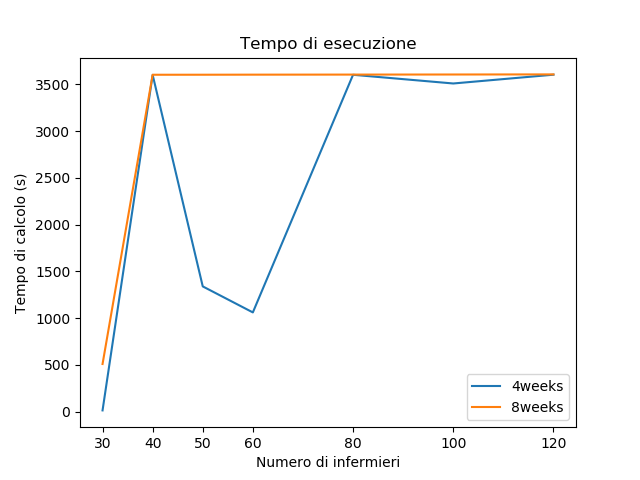
\includegraphics[scale=0.5]{img/Problema1/Time_1h-h0_w0.png}\\
  \caption{Tempo di esecuzione Problema 1}
\end{center}
\end{figure}

\begin{figure}[H]
\begin{center}
  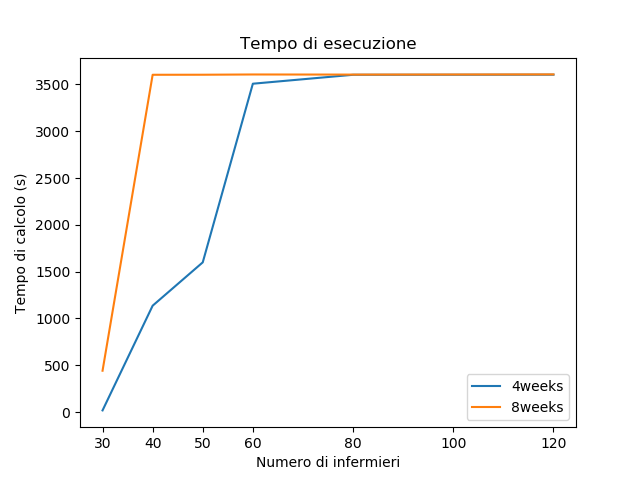
\includegraphics[scale=0.5]{img/Problema2/Time_1h-h0_w4.png}\\
  \caption{Tempo di esecuzione Problema 2}
\end{center}
\end{figure}

\begin{figure}[H]
\begin{center}
  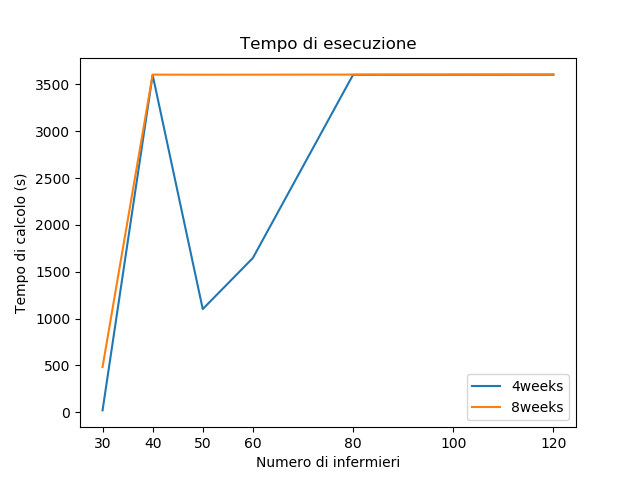
\includegraphics[scale=0.5]{img/Problema3/Time_1h-h1_w0.png}\\
  \caption{Tempo di esecuzione Problema 3}
\end{center}
\end{figure}

\begin{figure}[H]
\begin{center}
  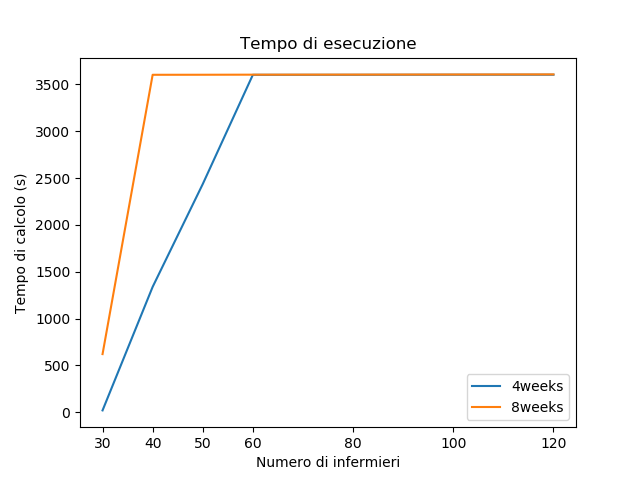
\includegraphics[scale=0.5]{img/Problema4/Time_1h-h1_w4.png}\\
  \caption{Tempo di esecuzione Problema 4}
\end{center}
\end{figure}


\subsection{Gap percentuale}
Di seguito si riportano i grafici nei quali si mostra il Gap percentuale del problema, dove si è posto un limite al tempo massimo di calcolo pari a 2 ore.
\begin{figure}[H]
\begin{center}
  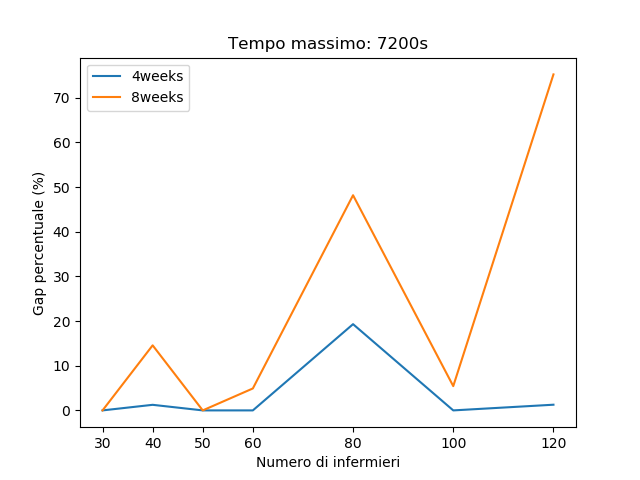
\includegraphics[scale=0.5]{img/Problema1/Gap_2h-h0_w0.png}\\
  \caption{Gap Problema 1}
\end{center}
\end{figure}

\begin{figure}[H]
\begin{center}
  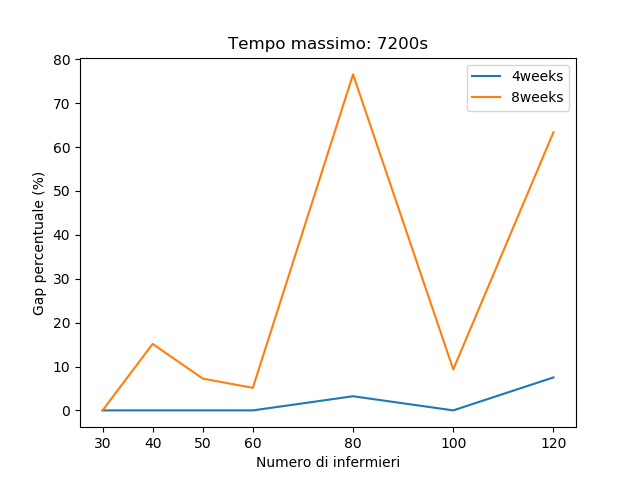
\includegraphics[scale=0.5]{img/Problema2/Gap_2h-h0_w4.png}\\
  \caption{Gap Problema 2}
\end{center}
\end{figure}

\begin{figure}[H]
\begin{center}
  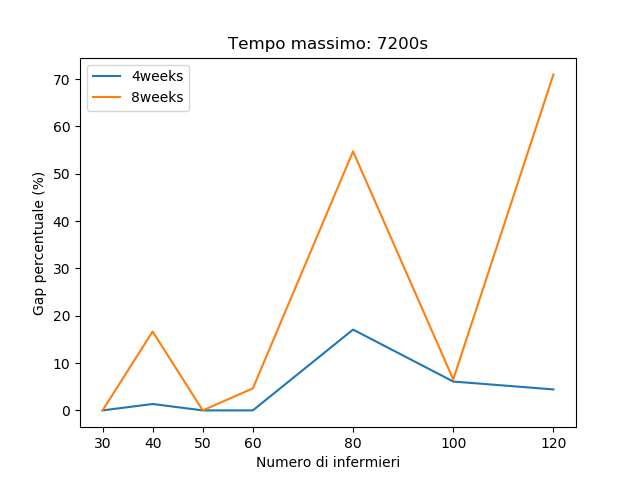
\includegraphics[scale=0.5]{img/Problema3/Gap_2h-h1_w0.png}\\
  \caption{Gap Problema 3}
\end{center}
\end{figure}

\begin{figure}[H]
\begin{center}
  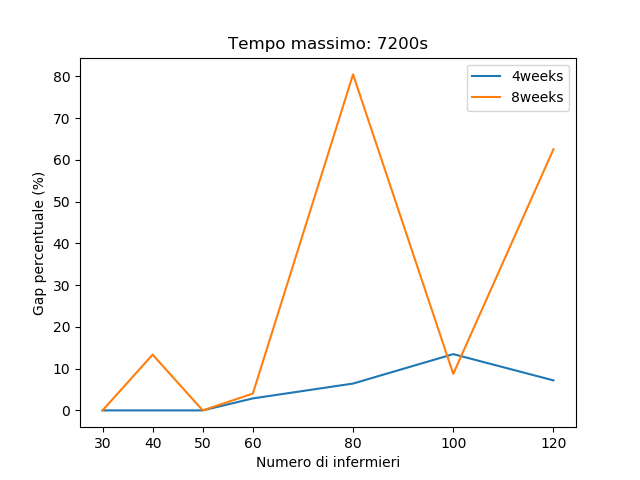
\includegraphics[scale=0.5]{img/Problema4/Gap_2h-h1_w4.png}\\
  \caption{Gap Problema 4}
\end{center}
\end{figure}

\newpage 
\section{Risultati}
Analizzando i grafici si possono fare le seguenti osservazioni:
\begin{itemize}
\item Il problema da 8 settimane appare molto più complesso da risolvere rispetto a quello di 4 settimane;
\item Il Gap del problema da 4 settimane non supera mai il 20\%;
\item Il Gap del problema da 8 settimane non supera mai l'80\%;
\item Il tempo di calcolo della soluzione arriva spesso in saturazione.
\end{itemize}

È necessario precisare che per eseguire una sperimentazione più precisa sarebbe stato opportuno fare una quantità maggiore di esperimenti facendo una media tra essi.

Si noti che, comunque, in tutti gli esperimenti fatti entro il tempo massimo, si riesce sempre a trovare una \textbf{soluzione} \textbf{ammissibile}.
\chapter{Interfaccia}\label{ch:chapter4}

\section{Introduzione}
Nonostante il nucleo principale di questa tesi fosse costruire il modello di ottimizzazione per la programmazione dei turni, è stata anche creata un'interfaccia base per mostrare un utilizzo vero e proprio del programma.
Per far questo è stato utilizzato Django, framework per Python, che ha permesso di sviluppare il lato server dell'applicazione \cite{ref:Django}.

Nella schermata principale è possibile visualizzare gli orari presenti nel database o crearne uno nuovo da zero. Selezionando un orario specifico è possibile, inoltre, visualizzarne i dettagli, come il numero di settimane e il numero di infermieri di cui si vuole gestire la pianificazione dei turni.
Inoltre, dato l'orario, per ogni tipologia di contratto presente è possibile assegnare differenti valori ad alcuni paramatri tra cui il numero minimo e massimo di giorni lavorativi/liberi consecutivi che un infermiere può svolgere.
È possibile inoltre specificare i dettagli di ogni infermiere, con le relative richieste che ognuno di essi può presentare. Infine, nella schermata finale, viene riportato l'output del programma.

\section{Orari}
\begin{figure}[H]
\begin{center}
  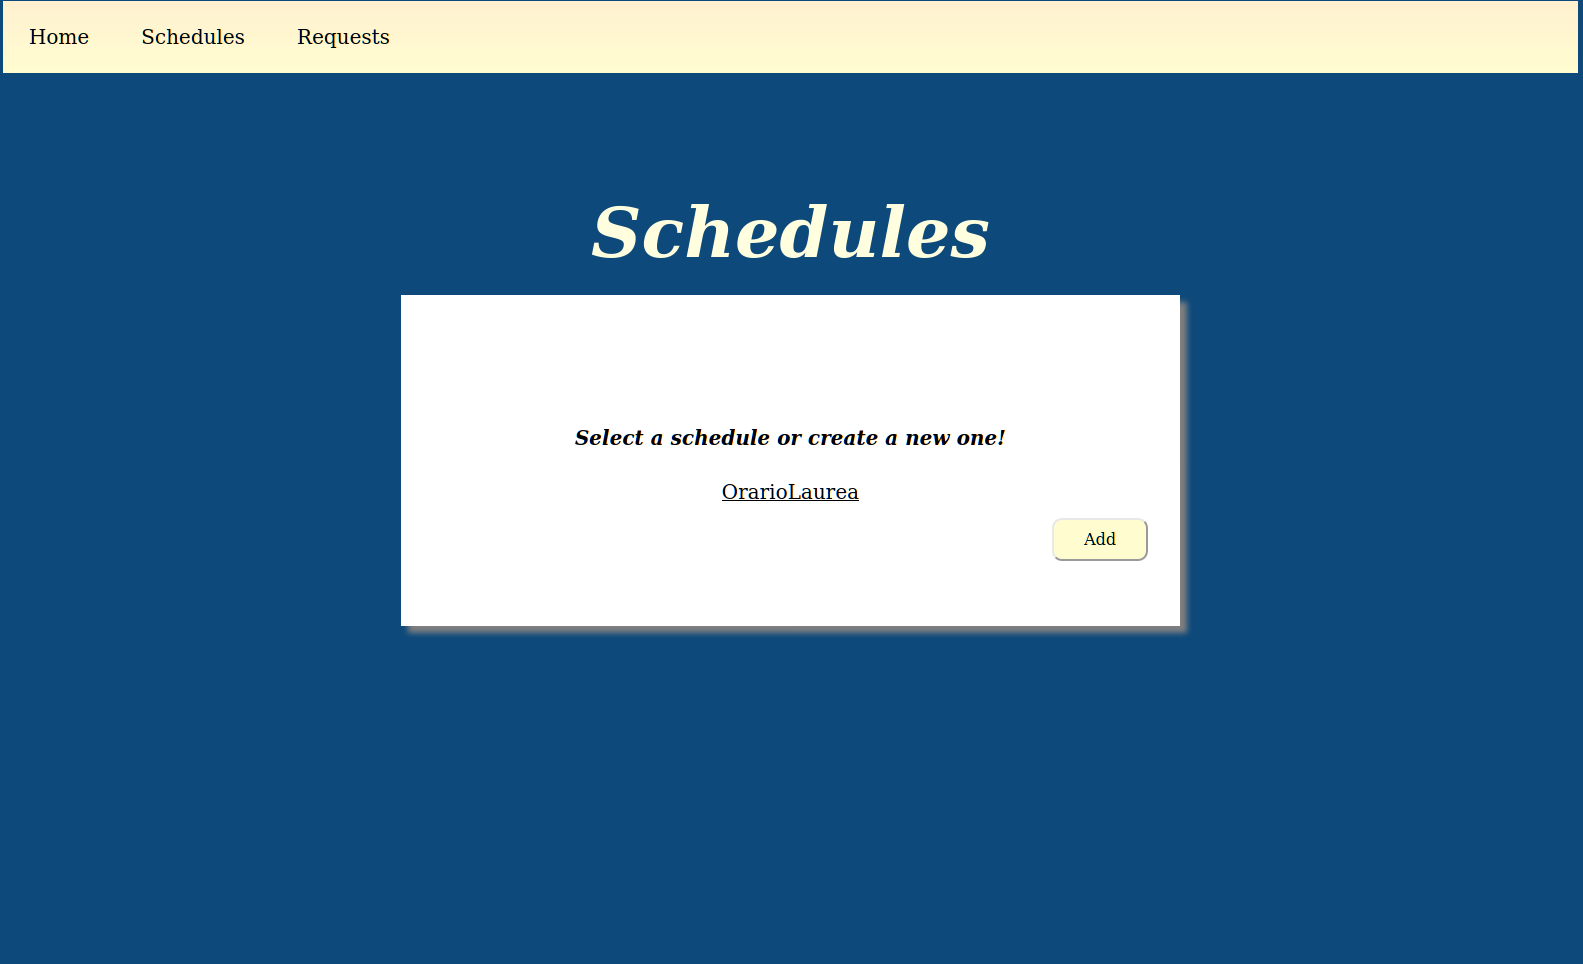
\includegraphics[scale=0.20]{img/Schermate/S1.png}\\
  \caption{Schermata Orari}
\end{center}
\end{figure}

\section{Dettagli Orario}
\begin{figure}[H]
\begin{center}
  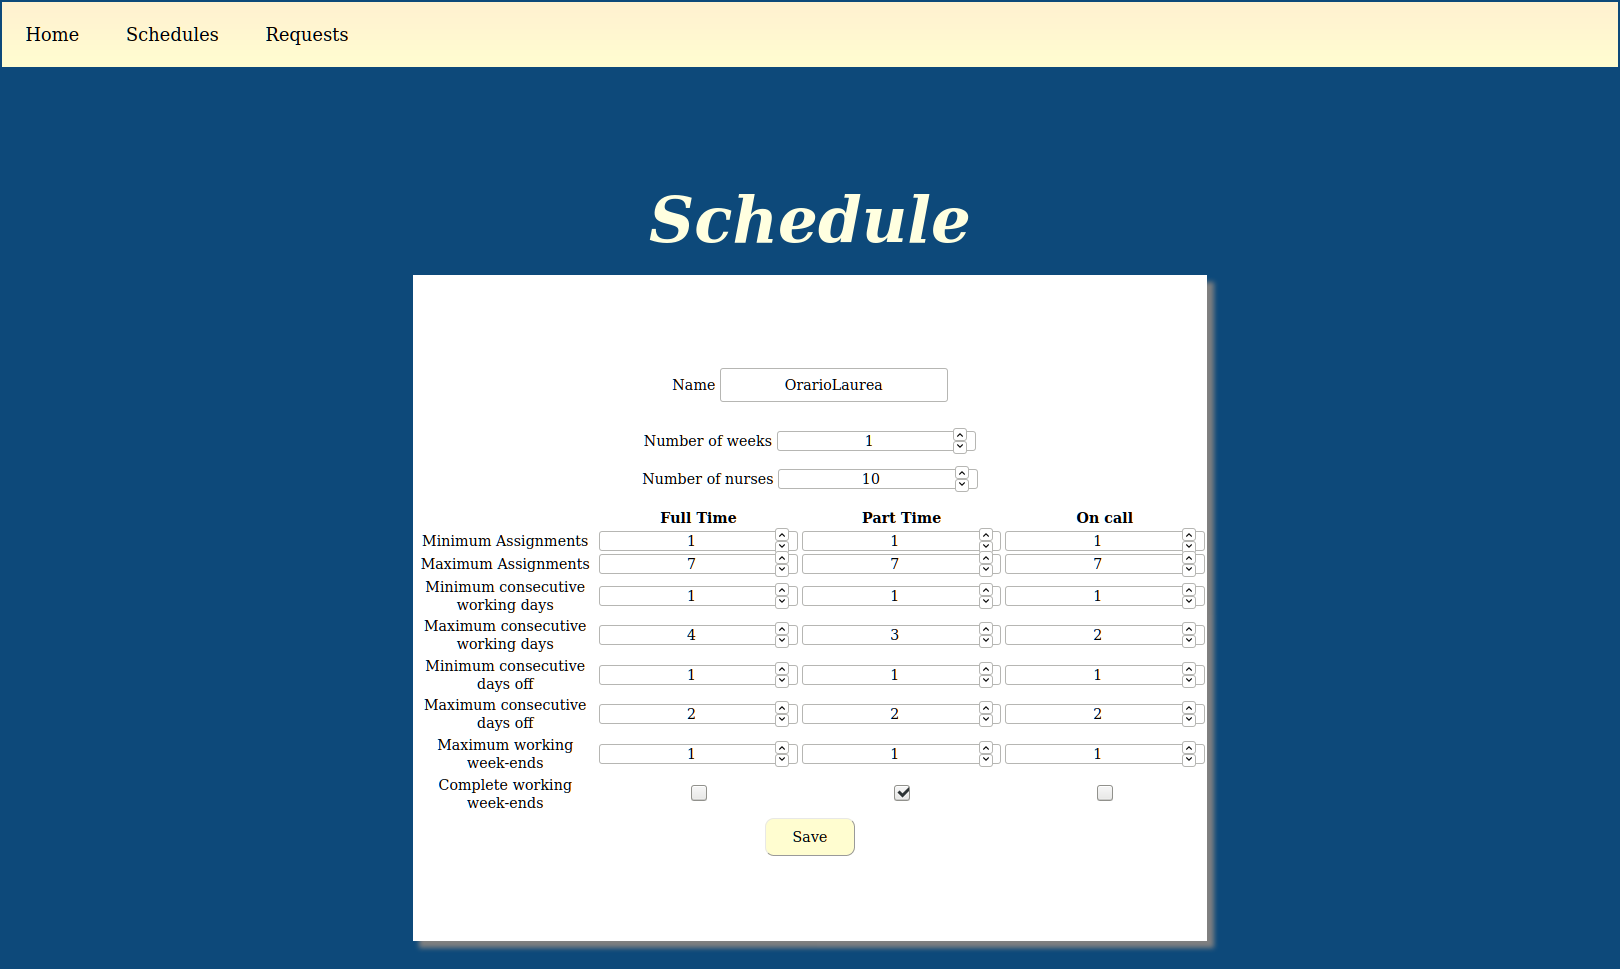
\includegraphics[scale=0.20]{img/Schermate/S2.png}\\
  \caption{Schermata dettagli Orario}
\end{center}
\end{figure}

\section{Dettagli Infermiere}
\begin{figure}[H]
\begin{center}
  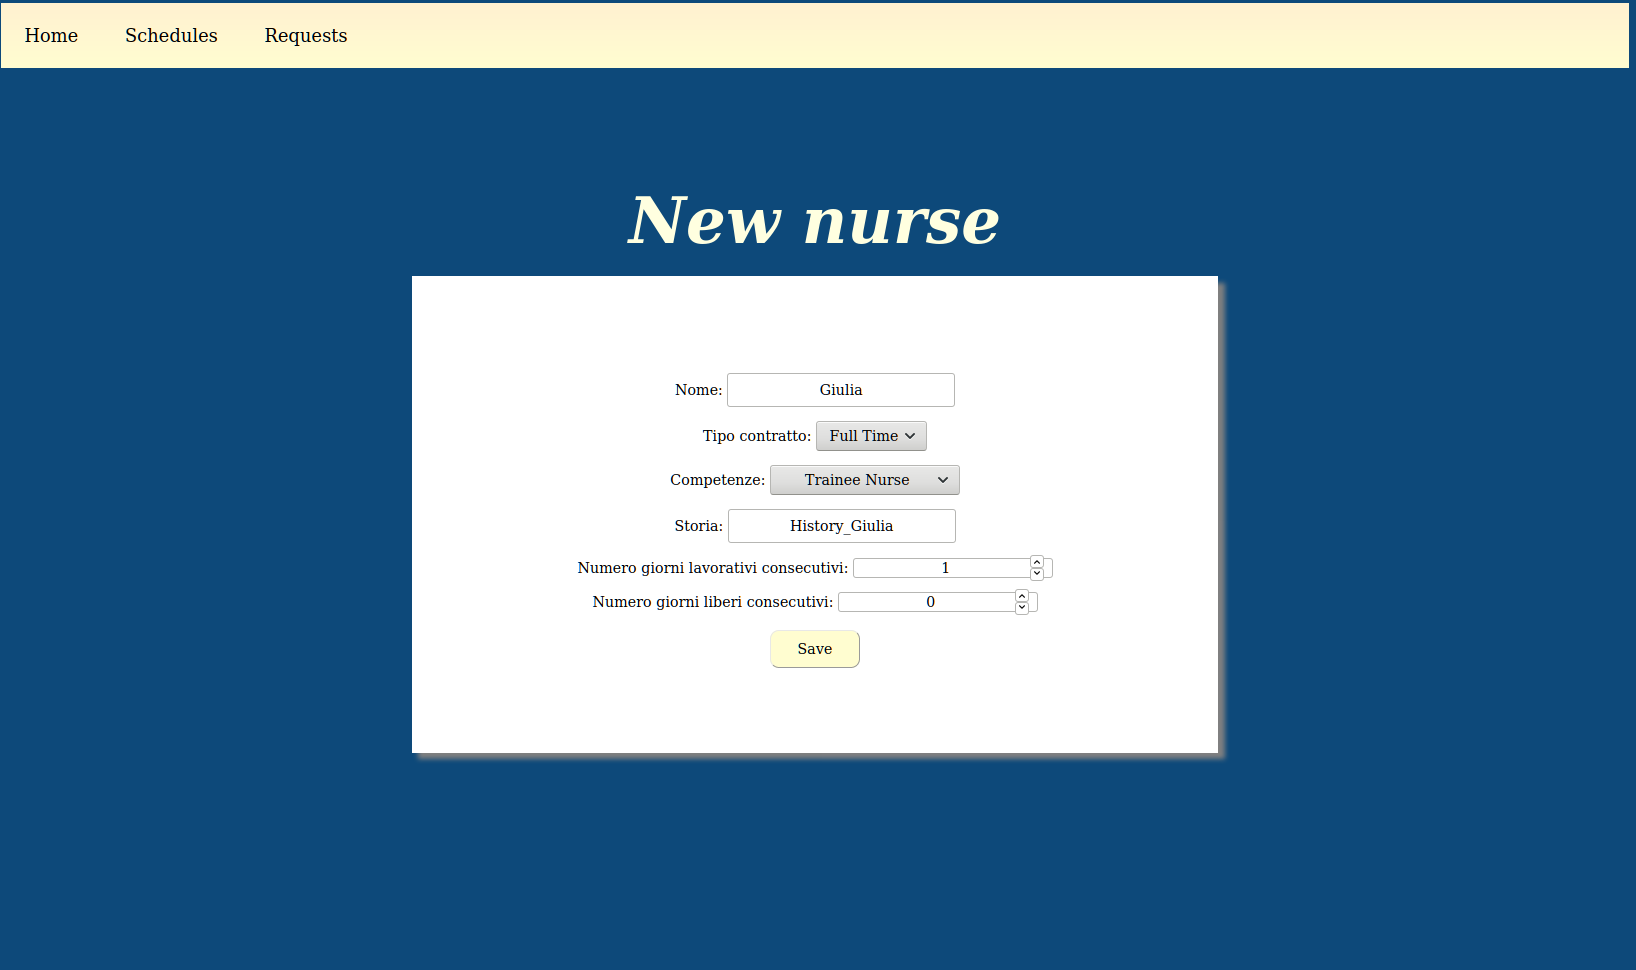
\includegraphics[scale=0.20]{img/Schermate/S5.png}\\
  \caption{Schermata dettagli Infermiere}
\end{center}
\end{figure}

\section{Richiesta Infermiere}
\begin{figure}[H]
\begin{center}
  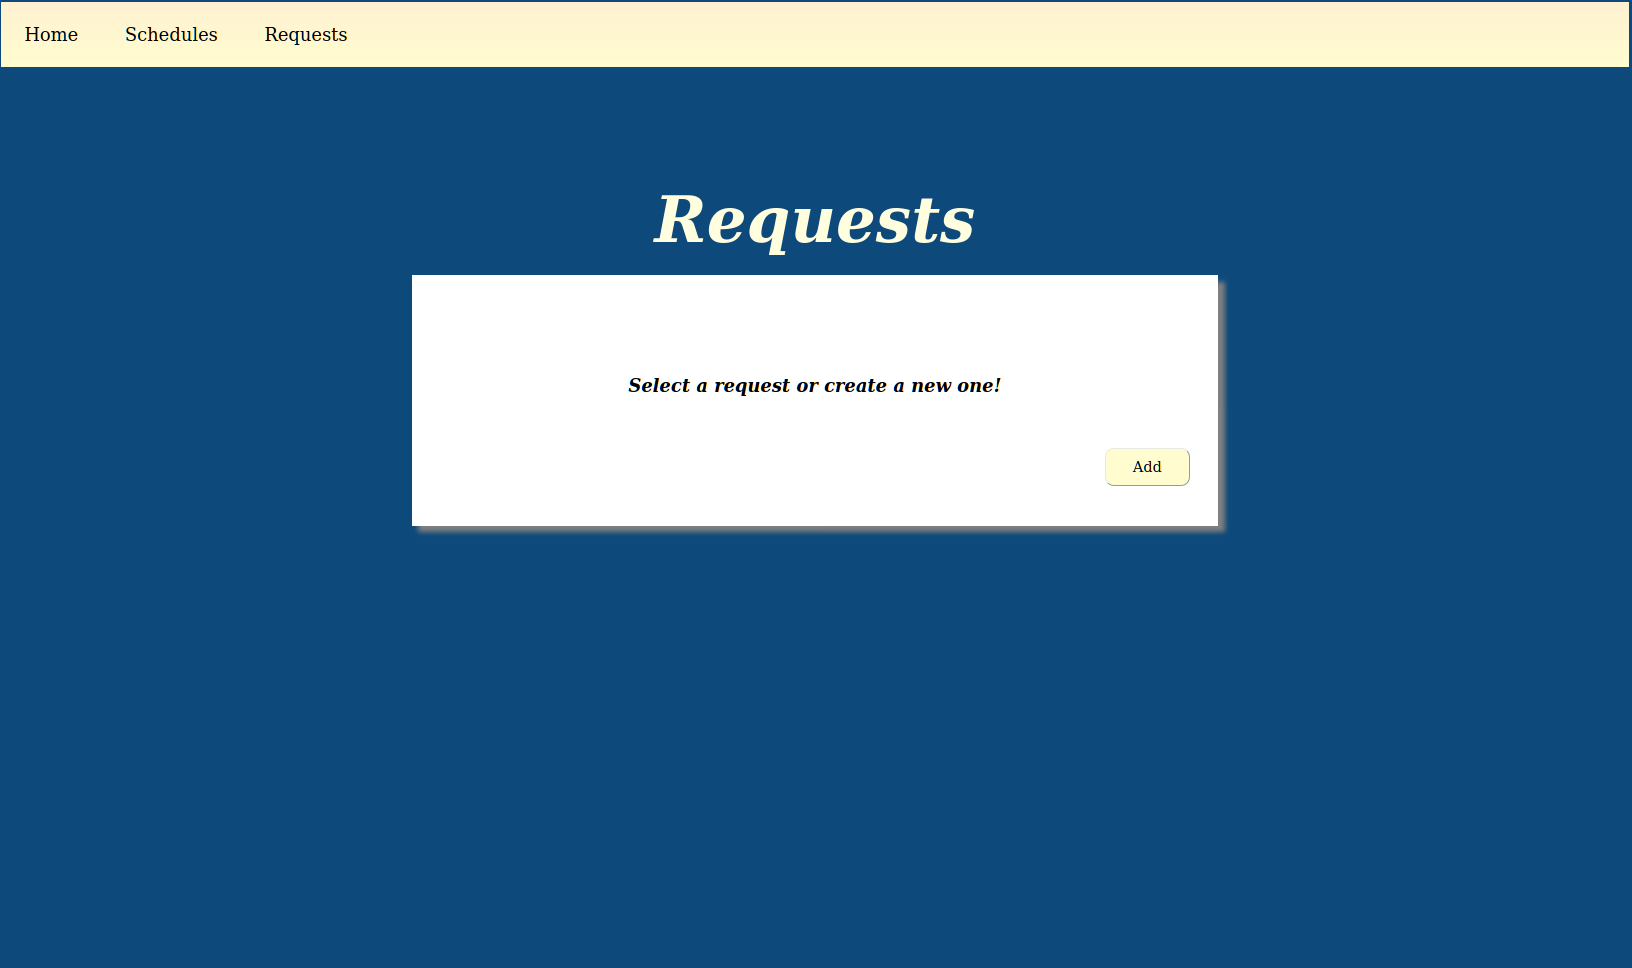
\includegraphics[scale=0.20]{img/Schermate/S3.png}\\
  \caption{Schermata Richieste}
\end{center}
\end{figure}

\begin{figure}[H]
\begin{center}
  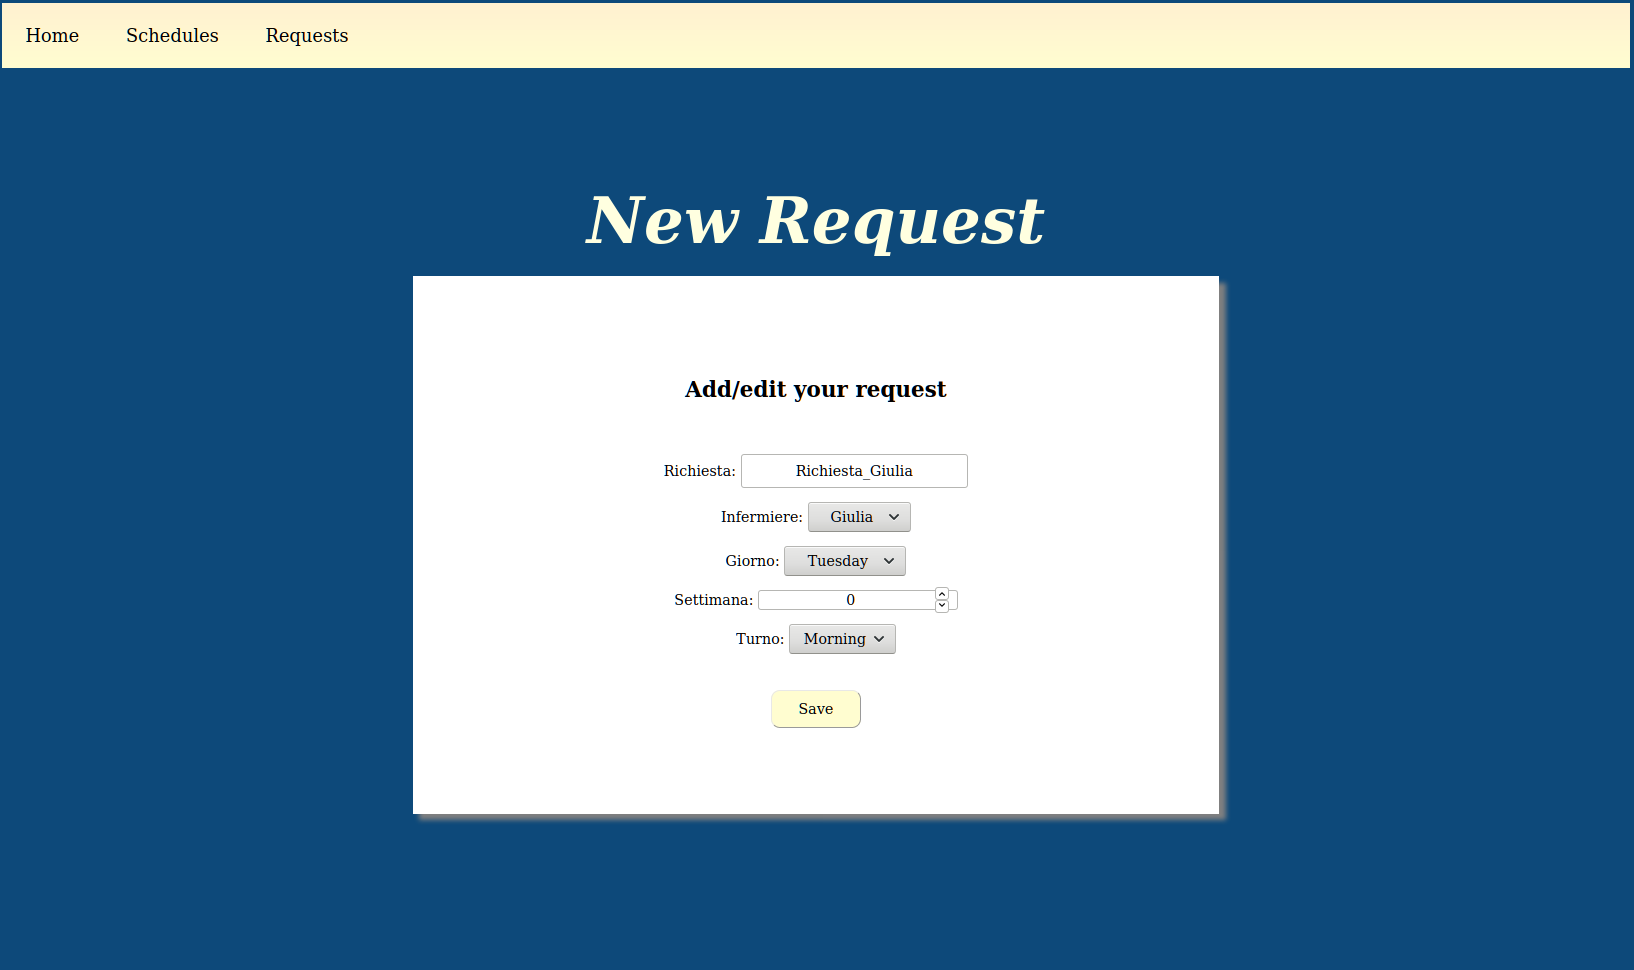
\includegraphics[scale=0.20]{img/Schermate/S4.png}\\
  \caption{Schermata richiesta Infermiere}
\end{center}
\end{figure}

\section{Risultato}
\begin{figure}[H]
\begin{center}
  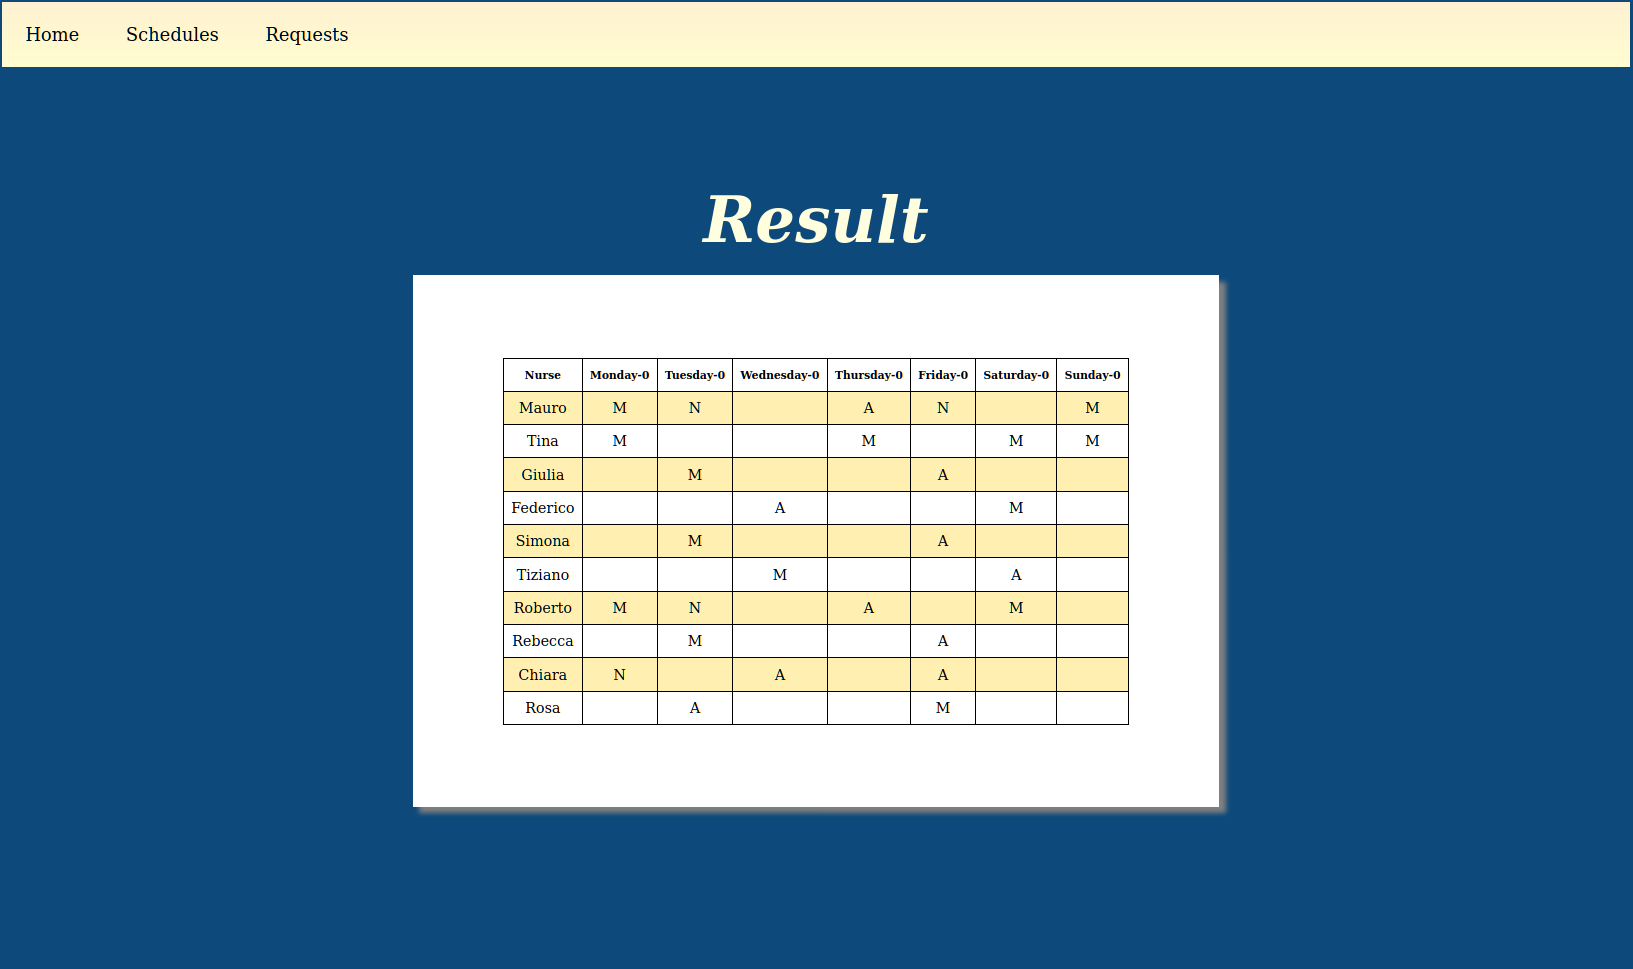
\includegraphics[scale=0.20]{img/Schermate/Result.png}\\
  \caption{Schermata Risultato}
\end{center}
\end{figure}

\chapter{Conclusioni}\label{ch:conclusioni}
Il problema affrontato è di fondamentale importanza nell'ambito sanitario, e non solo.
Infatti una gestione automatica dei turni lavorativi può aiutare a semplificare la gestione degli orari del personale in qualunque ambito lavorativo, e rimane particolarmente utile soprattutto in ambienti dove è richiesto di gestire un'elevata quantità di personale.

Nonostante l'elevato numero di variabili in gioco e l'elevato numero di vincoli imposti sul problema di ottimizzazione, il modello creato riesce a trovare una buona soluzione ammissibile al problema in tempi molto brevi e accettabili. Si è riusciti, inoltre, a creare un interfaccia funzionante e usabile dal punto di vista dell'utente. 

Per perfezionare il lavoro fatto in questa tesi, si potrebbe ampliare il modello creato con lo scopo di gestire situazioni non trattate, facendo, quindi, in modo che il sistema implementi più funzionalità diventando più generico e completo possibile.


\appendix
\chapter{Gurobi}

\section{Introduzione a Gurobi}
L'ottimizzatore usato per la pianificazione dell'orario degli infermieri è Gurobi \cite{ref:Gurobi}, che è un solutore di ottimizzazione commerciale usato in vari tipi di programmazione: lineare, quadratica, quadratica vincolata, lineare e quadratica intera mista, quadratica intera mista vincolata.

Gurobi, il cui nome deriva dai nomi dei suoi fondatori (Zonghao Gu, Edward Rothberg e Robert Bixby), è stato introdotto nel 2008 e supporta una varietà di linguaggi di programmazione e modellazione, inclusi:
\begin{itemize}
\item Interfacce Object-Oriented per C++, Java, .NET e Python;
\item Interfacce Matrix-Oriented per C, MATLAB e R;
\item Collegamenti a linguaggi di modellazione standard: AIMMS, AMPL, GAMS e MPL.
\end{itemize}

È possibile capire il ruolo di questo ottimizzatore dallo schema sottostante (Figura \ref{fig:Gurobi}).
\begin{figure}[!h]
		\centering
		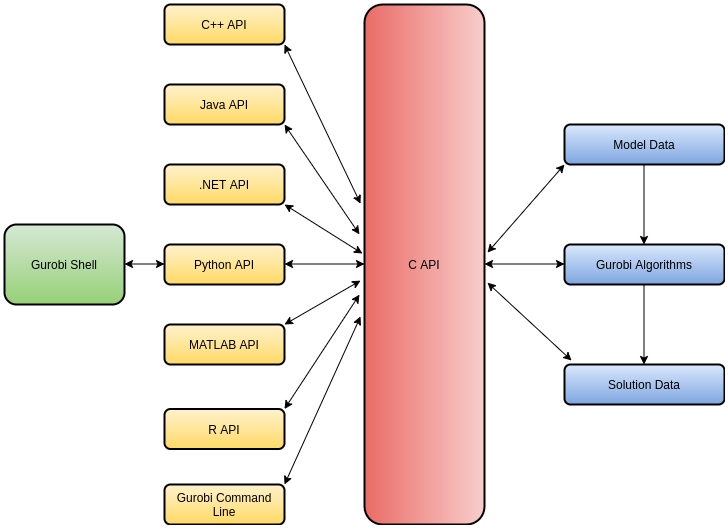
\includegraphics[scale=0.5]{img/gurobi_c.png}
		\caption{Gurobi API}
		\label{fig:Gurobi}
\end{figure}

\section{Principali API per Python}
In questa sezione vengono spiegate le funzionalità principali di Gurobi per il linguaggio Python, per dare una visione generale al lettore di come è possibile modellare un problema di ottimizzazione usando questo tipo di ottimizzatore.

%\subsection{Modello}

\subsection{Variabili}
Le variabili di decisione rappresentano il risultato dell'ottimizzazione.
In una soluzione ammissibile, i valori calcolati per le variabili di decisione soddisfano tutti i vincoli del modello. Alcuni di questi vincoli sono associati a singole variabili, mentre altri rappresentano relazioni tra esse.
Ci sono varie tipologie di variabili disponibili tra cui: continue, intere o intere binarie.

%\subsubsection*{Variabili continue}
%Le variabili continue possono assumere qualsiasi valore tra il loro limite inferiore e quello superiore. Nella programmazione matematica, la convenzione è che le variabili sono non negative se non diversamente indicato, quindi se non si forniscono esplicitamente i limiti per una variabile, si dovrebbe presumere che il limite inferiore sia 0 e quello superiore sia $\infty$. Una variabile con limiti superiori e inferiori uguali ad $\infty$ vine detta variabile libera.
%Inoltre le variabili possono violare i loro limite di tolleranza, che in questo caso è \texttt{FeasibilityTol}. È possibile ridurre questo valore, ma a causa di errori numerici potrebbe non essere possibile ottenere la precisione desiderata.
%
%\subsubsection*{Variabili intere}
%Le variabili intere, in generale, sono maggiormente vincolate rispetto a quelle continue, infatti possono assumere solo valori interi. 
%
%????
%
%In particolare i limiti inferiore e superiore di una ....
%Una soluzione non è considerata ammissibile a meno che tutte le variabili 
%
%\subsubsection*{Variabili binarie}
%Le variabili binarie sono particolari variabili intere che possono assumere solo valori pari a 0 o ad 1.
%Ancora una volta, a causa dei limiti dell'aritmetica a precisione finita, le variabili binarie assumeranno spesso valori che non sono esattamente....
%L'entità della violazione di integrità consentita è controllata dal parametro \texttt{IntFeasTol}.
%
%\subsubsection*{Variabili semi-continue e semi-intere}
%Le variabili semi-continue possono assumere valori pari a 0 o ad un valore compreso tra i limiti inferiore e superiore specificati.
%Una variabile semi-intera può assumere anche un valore intero.
%
%Entrambi questi tipi di variabili possono violare queste restrizioni, in questo caso la tolleranza pertinente è \texttt{IntFeasTol}.

\subsubsection*{Metodo per aggiungere variabili al modello}
Per aggiungere una nuova variabile al modello creato è necessario usare il metodo \texttt{addVar()}, il quale se ritorna un valore diverso da 0 indica che si è verificato un problema durante l'aggiunta della variabile.
Gli argomenti che possiamo specificare in questo metodo sono:
\begin{itemize}
\item \texttt{model}: modello al quale la variabile è aggiunta;
\item \texttt{lb}: lower bound;
\item \texttt{ub}: upper bound;
\item \texttt{obj}: coefficiente obbiettivo;
\item \texttt{vtype}: tipologia della variabile in questione;
le opzioni sono:
\begin{itemize}
\item \texttt{GRB\_CONTINUOUS};
\item \texttt{GRB\_BINARY};
\item \texttt{GRB\_INTEGER};
\item \texttt{GRB\_SEMICONT};
\item \texttt{GRB\_SEMINT}.
\end{itemize}
\item \texttt{varname}: nome della variabile.
\end{itemize}

Si riporta un esempio per illustrare l'uso di questo metodo:\\
\texttt{x = model.addVar(0.0, 1.0, 0.0, GRB.BINARY, name=`x')}\\
In questo caso il primo e il secondo argomento sono, rispettivamente, il limite inferiore e superiore della variabile x. Il terzo argomento rappresenta il coefficiente di obbiettivo lineare. Successivamente viene specificato il tipo della variabile (binaria), e come ultimo argomento ne viene indicato il nome.

Nel caso si vogliano aggiungere più variabili dello stesso tipo si può usare il metodo \texttt{addVars()}.

Si noti che con entrambi questi metodi le nuove variabili non vengono effettivamente aggiunte fino a quando non si aggiorna il modello, non lo si ottimizza o non lo si  scrive su disco.

\subsection{Vincoli}
Un vincolo rappresenta una restrizione sui valori che un insieme di variabili può assumere. Vi sono varie tipologie di vincoli disponibili: lineare, quadratico, SOS, generale.

\subsubsection*{Vincoli lineari}
Un vincolo lineare consente di limitare il valore di un'espressione lineare.
Un semplice esempio può essere il seguente:
$3x + 4y ~ \leq ~ 5z$

Si noti che le API Gurobi orientate alla matrice (C, MATLAB e R) richiedono che il lato destro di un vincolo sia una costante, mentre le API orientate agli oggetti (C++, Java, .NET e Python) consentono arbitrari espressioni lineari in entrambi i membri della comparazione.

Gurobi supporta un set limitato di comparatori: in particolare, è possibile vincolare un'espressione a essere minore o uguale, maggiore o uguale o semplicemente uguale ad un'altra. Invece non vengono supportati i comparatori di minore e maggiore stretto o il comparatore di disuguaglianza. 

\subsubsection*{Vincoli SOS}
Un vincolo SOS (insieme ordinato speciale) è un vincolo altamente specializzato che pone restrizioni ai valori che possono assumere le variabili in un determinato \textbf{elenco}.
Esistono due tipi di vincoli SOS:
\begin{itemize}
\item \textit{Vincolo SOS di tipo 1}: in cui al massimo una variabile nell'elenco specificato può assumere un valore diverso da 0;
\item \textit{Vincolo SOS di tipo 2}: al massimo due variabili nell'elenco specificato e ordinato possono assumere un valore diverso da 0 e tali variabili devono essere contigue nell'elenco.
\end{itemize}
Le variabili di un vincolo SOS possono essere continue, intere o binarie.

Quindi un vincolo SOS è descritto da un elenco di variabili e un elenco di pesi corrispondenti che servono per ordinare l'elenco delle variabili in questione.

\subsubsection*{Vincoli quadratici}
Un vincolo quadratico consente di limitare il valore di un'espressione quadratica.
Un esempio è il seguente:
$3x^2 + 4y^2 + 5z ~ \leq ~ 10$.

I vincoli quadratici sono spesso molto più difficili da soddisfare rispetto a quelli lineari. ma Gurobi può gestire sia quelli convessi che non.
Tuttavia gli algoritmi predefiniti di Gurobi accettano solo alcune \textbf{forme di vincoli quadratici}, noti per avere regioni convesse realizzabili.
%come per esempio quelle elencate qui di seguito:
%\begin{itemize}
%\item $x^T Q x + q^T x ~ \leq ~ b$;
%\item $x^T x ~ \leq ~ y^2$, dove x è un vettore di variabili e y una variabile non negativa;
%\item $x^T x ~ \leq ~ y z$, dove x è un vettore di variabili, e y e z sono variabili non negative.
%\end{itemize}
%Quindi verrà accettato un vincolo quadratico solo se si è in grado di trasformarlo in una di queste forme.

Si noti che altri risolutori quadratici non convessi spesso trovano solo soluzioni localmente ottime, invece gli algoritmi su cui si basa Gurobi esplorano l'intero spazio di ricerca, quindi forniscono un limite inferiore valido a livello globale e quindi, dato un tempo sufficiente, potranno trovare una soluzione ottima globale.

\subsubsection*{Vincoli generali}
I vincoli sopra descritti sono generalmente gestiti direttamente dagli algoritmi di ottimizzazione sottostanti. Gurobi include una serie aggiuntiva di vincoli, chiamati vincoli generali, progettati per una questione di praticità e funzionalità, in quanto permettono di definire facilmente determinate relazioni variabili.

Vi sono due tipologie di vincoli generali:
\begin{itemize}
\item \textit{Vincoli di funzione}, come per esempio $y ~ = ~ f(x)$, dove $x$ e $y$ sono due variabili decisionali e $f()$ è la funzione scelta in una lista di funzioni tra le seguenti: polinomiale, esponenziale, logaritmica, potenza, seno, coseno e tangente;
\item \textit{Vincoli semplici generali}, che consentono di stabilire relazioni comuni ma più dirette tra le variabili decisionali, e quelli supportati da Gurobi sono:
\begin{itemize}
\item vincolo \texttt{MAX}
\item vincolo \texttt{MIN}
\item vincolo \texttt{ABS}
\item vincolo \texttt{AND}
\item vincolo \texttt{OR}
\item vincolo \texttt{INDICATOR}
\item vincolo lineare a tratti
\end{itemize}
\end{itemize}

\subsubsection*{Metodo per aggiungere vincoli al modello}
Per aggiungere un nuovo vincolo al modello preso in esame viene usato il metodo \texttt{addConstr()}, dove i principali argomenti che accetta sono:
\begin{itemize}
\item \texttt{lhs}: membro sinistro del vincolo;
\item \texttt{rhs}: membro destro del vincolo;
\item \texttt{sense}: senso del vincolo, che può essere:
\begin{itemize}
\item \texttt{GRB.EQUAL};
\item \texttt{GRB.LESS\_EQUAL};
\item \texttt{GRB.GREATER\_EQUAL}.
\end{itemize}
\item \texttt{name}: nome de nuovo vincolo.
\end{itemize}

Un esempio dell'utilizzo di questo metodo è il seguente:\\
\texttt{model.addConstr(x + 2y, GRB.EQUAL, 3Z, name=`C\_0')}

\subsection{Funzione obbiettivo}
Ogni modello di ottimizzazione ha una funzione obbiettivo, che è la funzione definita mediante le variabili decisionali che si desidera minimizzare o massimizzare.
La maggior parte dei problemi ha molteplici soluzioni ottimali, quella restituita da Gurobi dipende dal tipo di problema preso in esame.
In generale questo ottimizzatore restituisce un'unica soluzione ottimale per modelli continui e una sequenza di soluzioni migliorative per modelli discreti.

Gli algoritmi di Gurobi lavorano per risolvere un modello fino a quando non trovano una soluzione ottimale entro le tolleranze specificate.
Per modelli discreti, nonostante sia possibile chiedere al risolutore di trovare una soluzione con il miglior valore obbiettivo, è molto comune fermarsi quando l'obbiettivo della soluzione rientra in un intervallo specificato del valore ottimale.
Questo Gap dell'ottimalità è controllato dal parametro \texttt{MIPGap} il cui valore predefinito è 0,01\%.

Le funzioni obbiettivo possono essere: lineari, quadratiche, lineare a tratti e multi-obbiettivo lineari.

\subsubsection*{Metodi principali della funzione obbiettivo}
Per impostare l'obbiettivo del modello uguale ad un'espressione lineare o quadratica viene usato il metodo \texttt{setObjective()}, che ha come parametri:
\begin{itemize}
\item \texttt{linExpr} o \texttt{quadExpr}: espressione lineare o quadratica:
\item \texttt{sense}: si può specificare se si desidera minimizzarla o massimizzarla.
\end{itemize}

Per esempio sia $f(x)$ la funzione obbiettivo, supponiamo di volerla minimizzare:\\
\texttt{model.setObjective($f(x)$, GRB.MINIMIZE)}\\
Una volta settata la funzione obbittivo per minimizzarla è necessario richiamare il metodo \texttt{optimize()} sul modello in questione:\\
\texttt{model.optimize()}


\addcontentsline{toc}{chapter}{Bibliografia}
\bibliographystyle{plain}
\bibliography{files/biblio}
\chapter*{Ringraziamenti}\label{ch:ringraziamenti}
Per concludere vorrei ringraziare in primis il Professor Fabio Schoen, relatore di questa tesi di laurea, e il Dottor Matteo Lapucci, correlatore, senza i quali questo lavoro non sarebbe stato possibile.\\

Inoltre vorrei ringraziare i miei genitori per avermi sempre sostenuta e per avermi permesso di portare a termine questo primo ciclo dei miei studi universitari, senza farmi mancare mai niente.
Grazie di cuore anche a tutti gli altri componenti della mia famiglia, a mio zio Roberto, e alle mie cugine Chiara e Rebecca, e a tutti i miei amici più fidati.\\

Un ringraziamento sincero al mio amato amico felino, Merlino, che mi ha sempre accompagnata nelle serate di studio intenso.\\

Infine un ringraziamento speciale va al mio ragazzo, Federico, detto anche "Il grande Capo", da cui ho imparato tantissimo, il quale mi ha sempre supportato e sopportato credendo in me anche quando nemmeno io ci credevo. Grazie per ogni singola volta che mi hai aiutata e spronata mostrandomi tutto il tuo amore.\\

\begin{center}
Grazie di cuore a tutti.
\end{center}
\bibliographystyle{unsrt}
%\bibliography{sp,xml}

\end{document} 